\section{DESARROLLO DE LA APLICACIÓN}

El objetivo de este capítulo es presentar el desarrollo de la aplicación pasando por el \textit{framework} metodológico adoptado en la tesis. Aquí, definen las épicas\footnote{Épica puede ser vista como una historia de usuario de alta complejidad (petición de negocio de alto nivel y complejidad, no clara), sacado de \url{http://diegoacosta.net/blog/2017/12/10/scrum-con-jira-relacion-entre-epicas-historias-y-tareas-tecnicas/}} con sus respectivas historias de usuario, para finalmente definir la cantidad de sprint necesarias para obtener el mínimo producto viable de la aplicación. En el mismo capítulo se presenta como se conformó el equipo y estructura utilizando la metodología Scrum. 

\subsection{\textit{FRAMEWORK} AGILE}

Hoy en día existen muchos \textit{framework} para el desarrollo de \textit{software}, sin embargo para la construcción de la aplicación D-Minute hemos seleccionado algunos de los artefactos y ritos de Scrum \fullcite{RN33} dada sus ventajas y familiarización que tiene el team de desarrollo. Es importante mencionar que Scrum (ver figura \ref{img4-1}) es uno de los framework más utilizados en la industria del \textit{software} a nivel mundial\footnote{Tomado de: \url{https://www.forbes.com/sites/stevedenning/2015/07/23/the-worlds-most-popular-innovation-engine/\#25f09da7c769}}, algunas de sus ventajas\footnote{Tomado de: \url{https://alfatecsistemas.es/los-10-beneficios-la-metodologia-scrum/} y \url{http://scrumguides.org/docs/scrumguide/v2017/2017-Scrum-Guide-US.pdf\#zoom=100}} son las siguientes:

\begin{enumerate}[1.]
    \item Fomenta la motivación y el compromiso del equipo 
    \item Provoca una mayor productividad al eliminar la burocracia.
    \item La organización horizontal promueve la autonomía y la auto-organización.
    \item El desglose del trabajo favorece a una mayor flexibilidad a los cambios. 
    \item Este trabajo intensificado conlleva una alta predicción de tiempos puesto que se conoce la velocidad y rendimiento del equipo.
    \item Dominar estos rasgos del equipo de trabajo reduce los riesgos al conocer las funcionalidades de cada rol y la velocidad a la que avanza el proyecto.
    \item La capacidad de flexibilidad y la reducción de riesgos permiten cumplir las expectativas del cliente.
    \item También, reduce el Time to Market: el cliente puede empezar las funcionalidades principales del proyecto antes de que este esté acabado.
    \item El método de trabajo y la revisión continua produce una mayor calidad del \textit{software}.

\end{enumerate}

\begin{figure}[h]
\centering
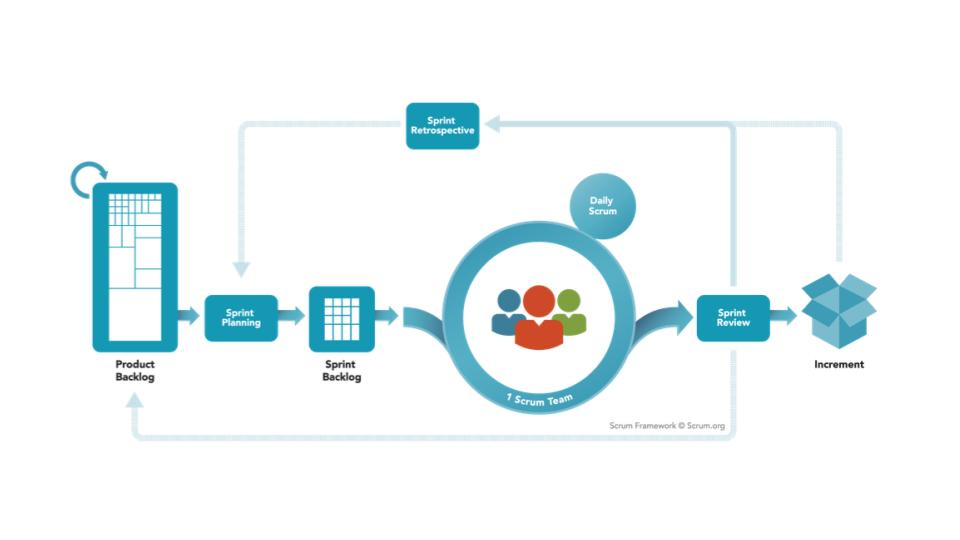
\includegraphics[width=1\linewidth]{/scrum}
\caption{Framework Scrum; tomado de Scrum.org} 
\label{img4-1}
\end{figure}

Si bien el \textit{framework} es una guía para la forma de abordar el desarrollo de la mejor manera, se requiere una herramienta para realizar la gestión respectiva del proyecto, para este caso se utilizó la plataforma online TAIGA\footnote{TAIGA: aplicación para seguimiento de proyectos ágiles, ver \url{https://taiga.io/}} (ver figura \ref{img4-2})

\begin{figure}[!h]
\centering
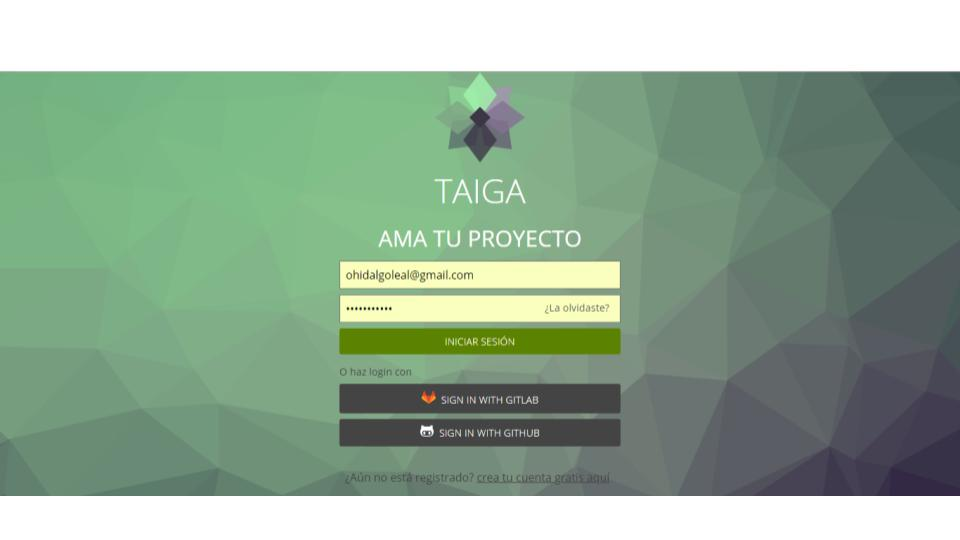
\includegraphics[width=12cm]{/taiga}
\caption{Vista principal de la plataforma para seguimiento proyecto; tomada de Taiga.io} 
\label{img4-2}
\end{figure}

\subsection{\textit{TEAM} DESARROLLO}

Scrum recomienda que un equipo “(...) debe ser pequeño como para permanecer ágil y lo suficientemente grande como para completar una cantidad significativa de trabajo” \fullcite{RN33}, pero no se recomienda más de nueve personas, dado lo anterior el equipo se conforma por cinco personas con diferentes roles (ver figura \ref{img4-3}).

\begin{figure}[!h]
\centering
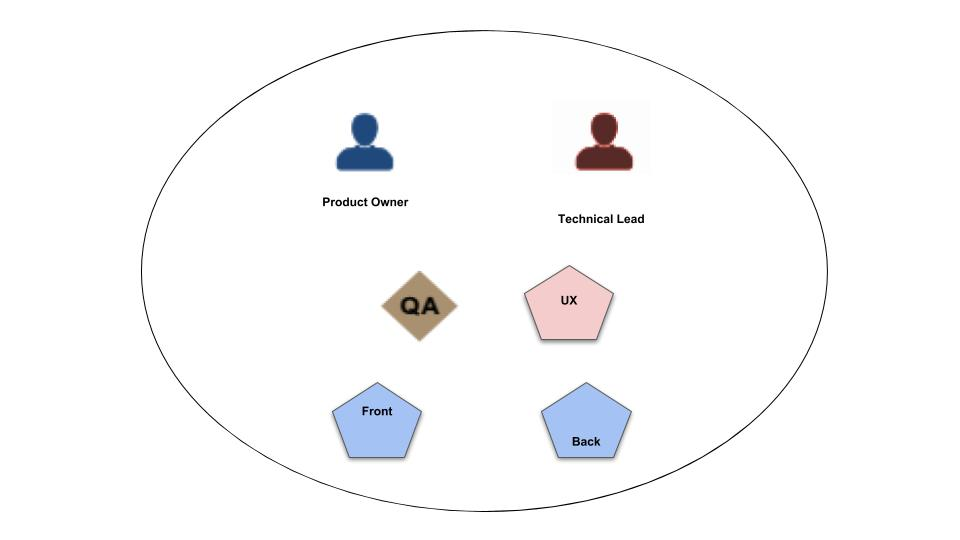
\includegraphics[width=10cm]{/equipo}
\caption{Estructura de equipo desarrollo y roles incorporados; elaboración propia} 
\label{img4-3}
\end{figure}

Si bien existe un equipo multidisciplinario, es importante indicar que a cada una de las personas individualizadas se les presentó el proyecto invitándolos a participar de esta iniciativa sin compromiso y sin un pago establecido. Los roles asumidos son los siguientes:

\begin{enumerate}[1.]
    \item Product Owner: Edmundo P. Leiva-Lobos (profesor guía)
    \item Technical Lead: Oliver Hidalgo (tesista)
    \item QA: Michele Fuenzalida
    \item Front: Francisco Gonzalez 
    \item Back: Andres Perez
    \item UX: Valentina Reyes
\end{enumerate}

Se debe subrayar que como tesista encargado del proyecto no solo organice el equipo de desarrollo. La mayoría de la programación, toda la integración e instalación del \textit{software} D-Minute en un servidor del departamento, fue de exclusiva responsabilidad del autor de esta tesis.

\subsection{ÉPICA}

Una epica es un concepto de agrupación  de funcionalidades que forma un macro requerimiento de negocio, esta puede contener muchas historias de usuarios que el equipo debe ir descomponiendo para lograr el desarrollo a un nivel de 80/20\footnote{ El concepto 80/20 indica que del 100\% de un producto sólo se ocupa el 20\% y el 80\% restante es desperdicio. Esto no es otra cosa que la aplicación de la famosa Ley de Pareto}. Para el proyecto en cuestión se identificaron los macro conceptos necesarios para obtener un MVP\footnote{MVP = Mínimo Producto Viable}, estas épicas se detallan y se muestran en figura \ref{img4-4}:

\begin{enumerate}[1.]
   \item Evolución UX: Corresponde a la línea gráfica desarrollada en la aplicación
   \item Deuda Técnica: Corresponde a las HDU técnicas que surgieron en el desarrollo de la aplicación
   \item Generación Acta: Corresponde a la funcionalidad completa de crear un acta
   \item Seguimiento de Tareas: Corresponde a la funcionalidad del seguimiento de los elementos del diálogo
   \item Trazabilidad elementos del diálogo: Corresponde al seguimiento de los elementos del diálogo una vez creados
\end{enumerate}

\begin{figure}[!h]
\centering
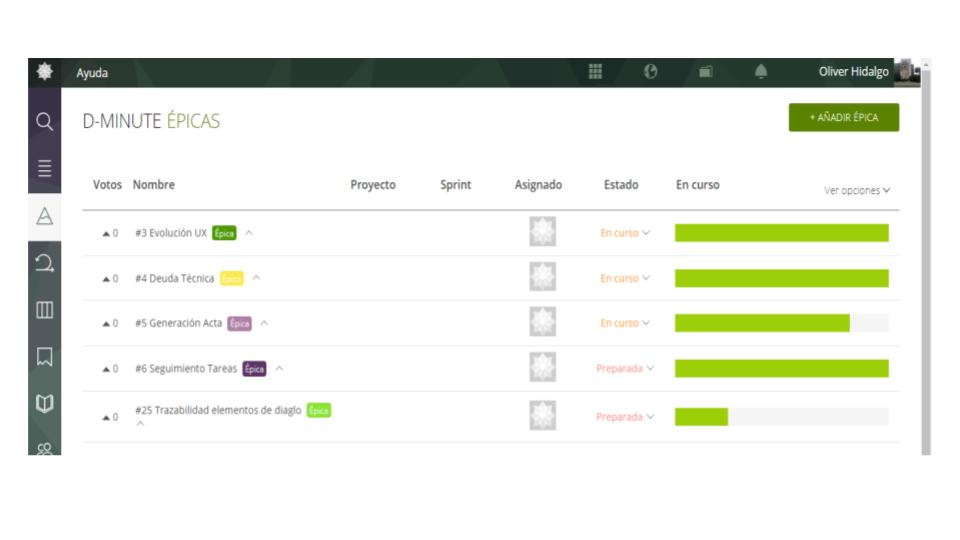
\includegraphics[width=12cm]{/epicas}
\caption{Épicas D-Minute; elaboración propia} 
\label{img4-4}
\end{figure}

\subsection{\textit{RELEASE MAP}}

Un \textit{release map} representa la visión general del proyecto dado los plazos fijos que se posee para llevar a cabo el desarrollo. Importante mencionar que el equipo puede ir tomando historias de usuario de diferentes épicas pues el objetivo es ir generando un \textit{software} funcionando en cada iteración y obtener feedback temprano del cliente, a continuación se presentan las épicas - en figura \ref{img4-5} - del producto que fueron planificadas al inicio del desarrollo:

\begin{figure}[!h]
\centering
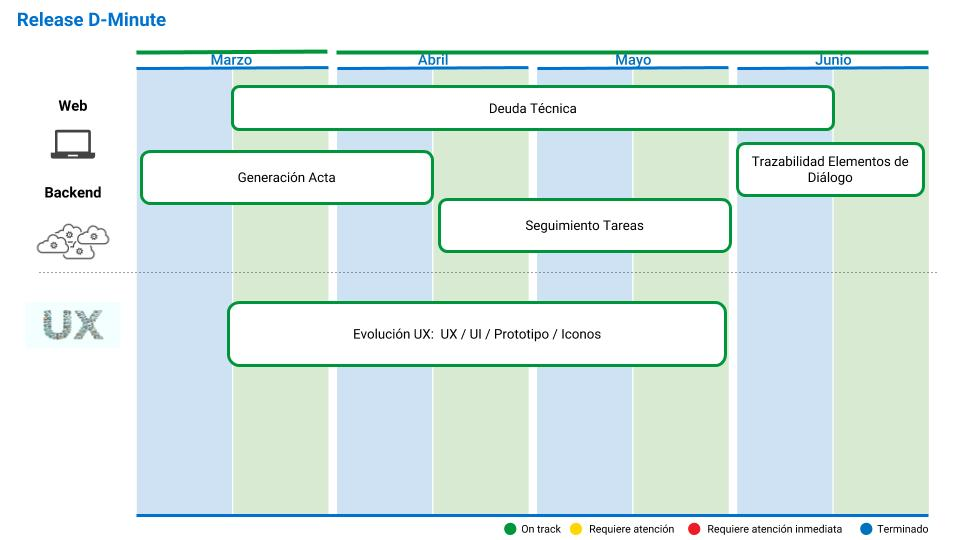
\includegraphics[width=12cm]{/releasemap}
\caption{\textit{Release Map} D-Minute; elaboración propia} 
\label{img4-5}
\end{figure}

\subsubsection{Duración de \textit{Sprint}}

Dado el análisis del equipo y los tiempos para llevar a cabo este desarrollo se definió que cada \textit{sprint} tendría una duración fija de dos semanas para permitir conocer la velocidad del equipo e ir ajustando en cada iteración. 	

\subsubsection{Cantidad de \textit{Sprint}}

La cantidad de \textit{sprint} está dada por el tiempo que se posee para el desarrollo del producto, para este caso se generaron ocho \textit{sprint}.

\subsubsection{Versión UX/UI}

D-Minute, es una aplicación que deriva de otra llamada meetingviewer que fue desarrollada por una alumna de ingeniería de la Universidad de Chile, como se menciona en el CAPÍTULO 1, que a su vez nace del prototipo desarrollado por Bossel en 2012. Si bien es un \textit{software} existente, no es una versión estable y lista de cara a clientes pues no posee las funcionalidades de forma correcta lo que genera un incorrecto uso de los elementos de diálogo. Es por esto que antes de comenzar a desarrollar D-Minute se trabajó con \textit{Lean} UX para mejorar\footnote{Línea gráfica puede verse en detalle en \url{https://app.zeplin.io/project/57fc415a616bae6b3307f637/dashboard}}: usabilidad, trazabilidad y buscabilidad de los elementos de diálogo.

La siguiente figura corresponde al bosquejo inicial de la aplicación que fue guía para el desarrollo de las siguientes maquetas (ver figura \ref{img4-6}).

\begin{figure}[!h]
\centering
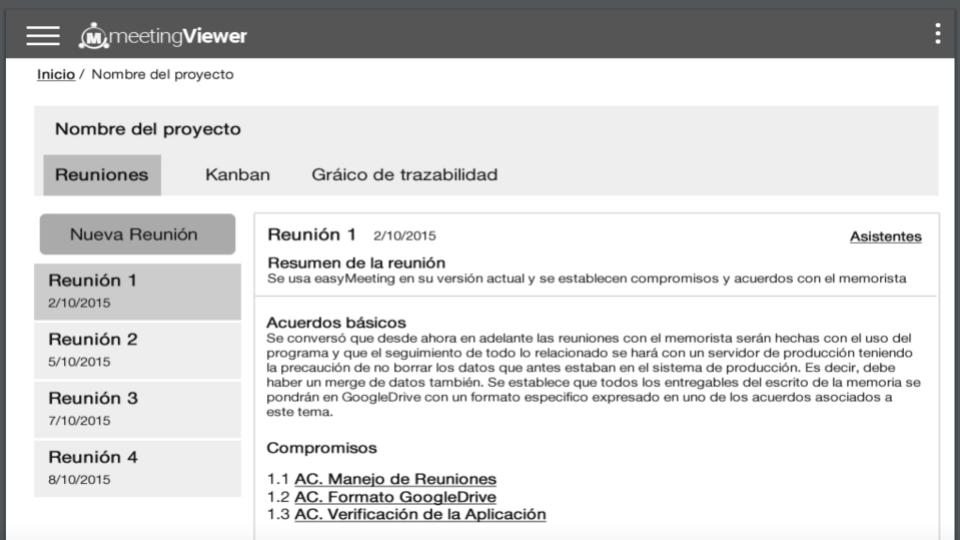
\includegraphics[width=12cm]{/versioninicial}
\caption{Bosquejo nuevo Diseño D-Minute; elaboración propia} 
\label{img4-6}
\end{figure}

Tomando de base el \textit{mockup} de la aplicación, se comenzó a desarrollar la cáscara del producto, partiendo por la figura siguiente que corresponde al \textit{login} de la aplicación futura (ver figura \ref{img4-7}).

\begin{figure}[!h]
\centering
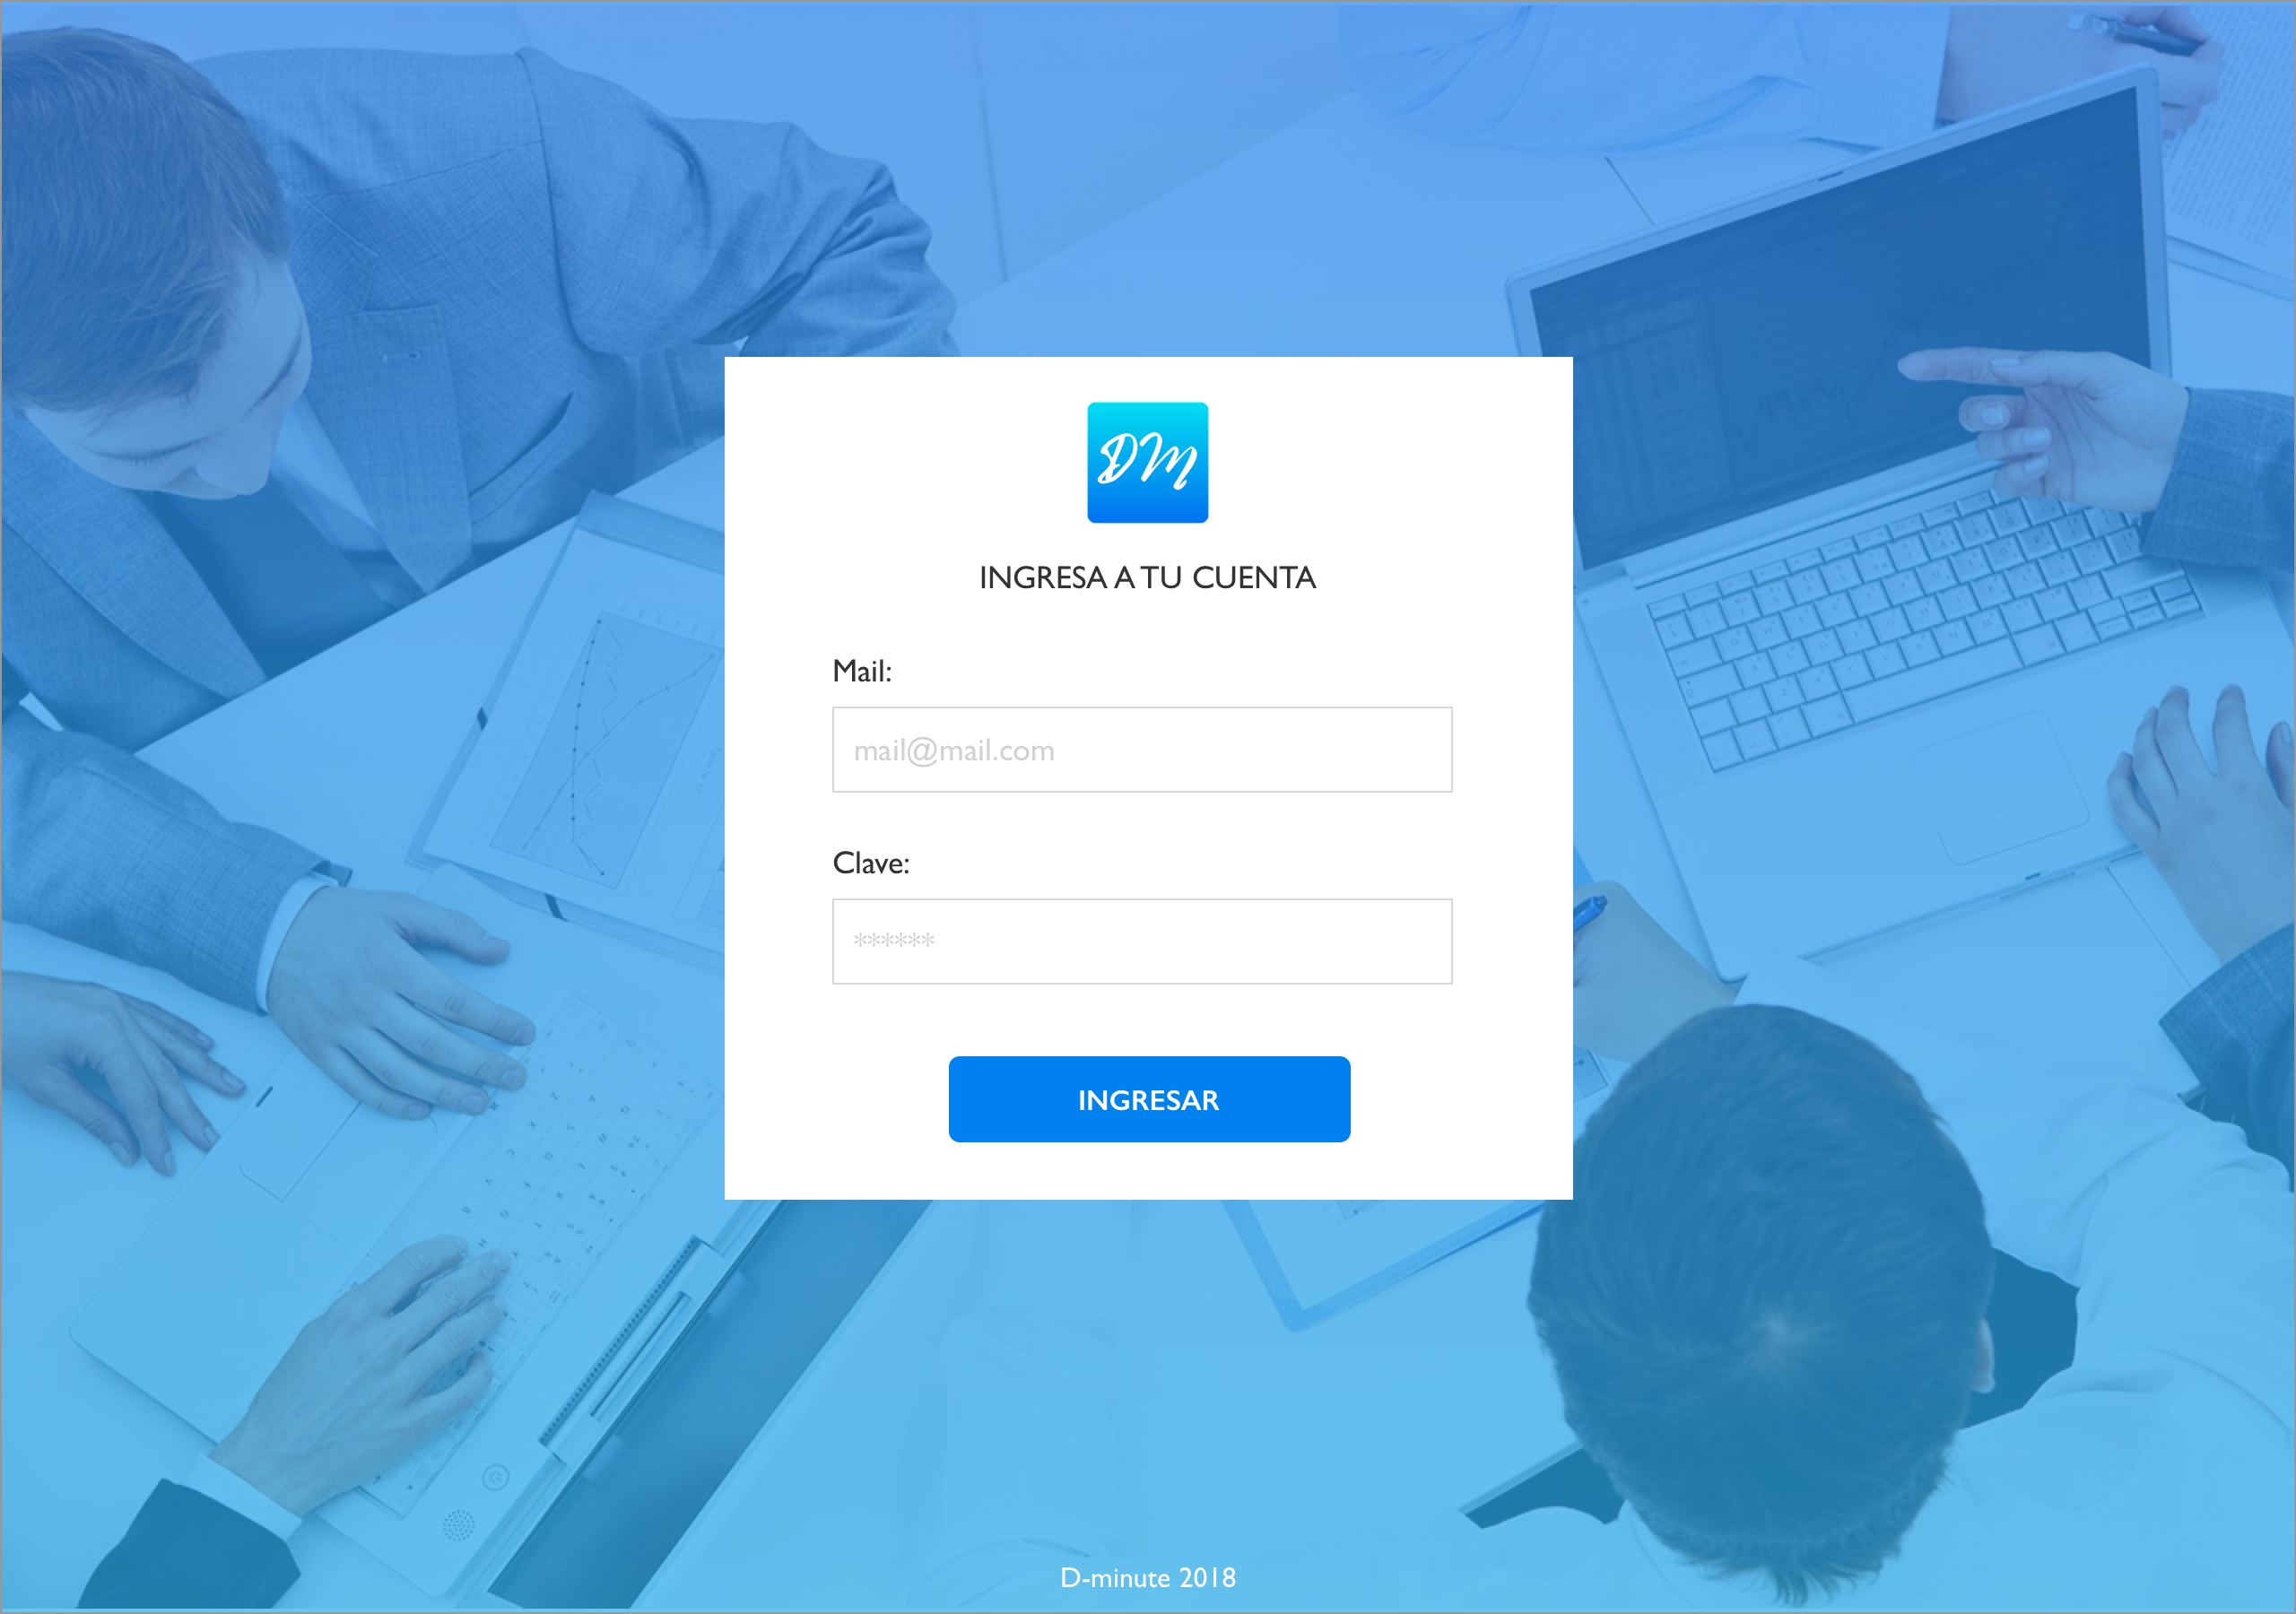
\includegraphics[width=11cm]{/app/Login_DMinute}
\caption{Diseño UX login D-Minute; elaboración propia} 
\label{img4-7}
\end{figure}

Una vez confeccionado el login fue posible establecer cuál sería el estilo de la aplicación y sus componentes asociados a utilizar, es por esto que la siguiente figura presenta cómo se vería la opción agregar proyecto (ver figura \ref{img4-8}).

\begin{figure}[!h]
\centering
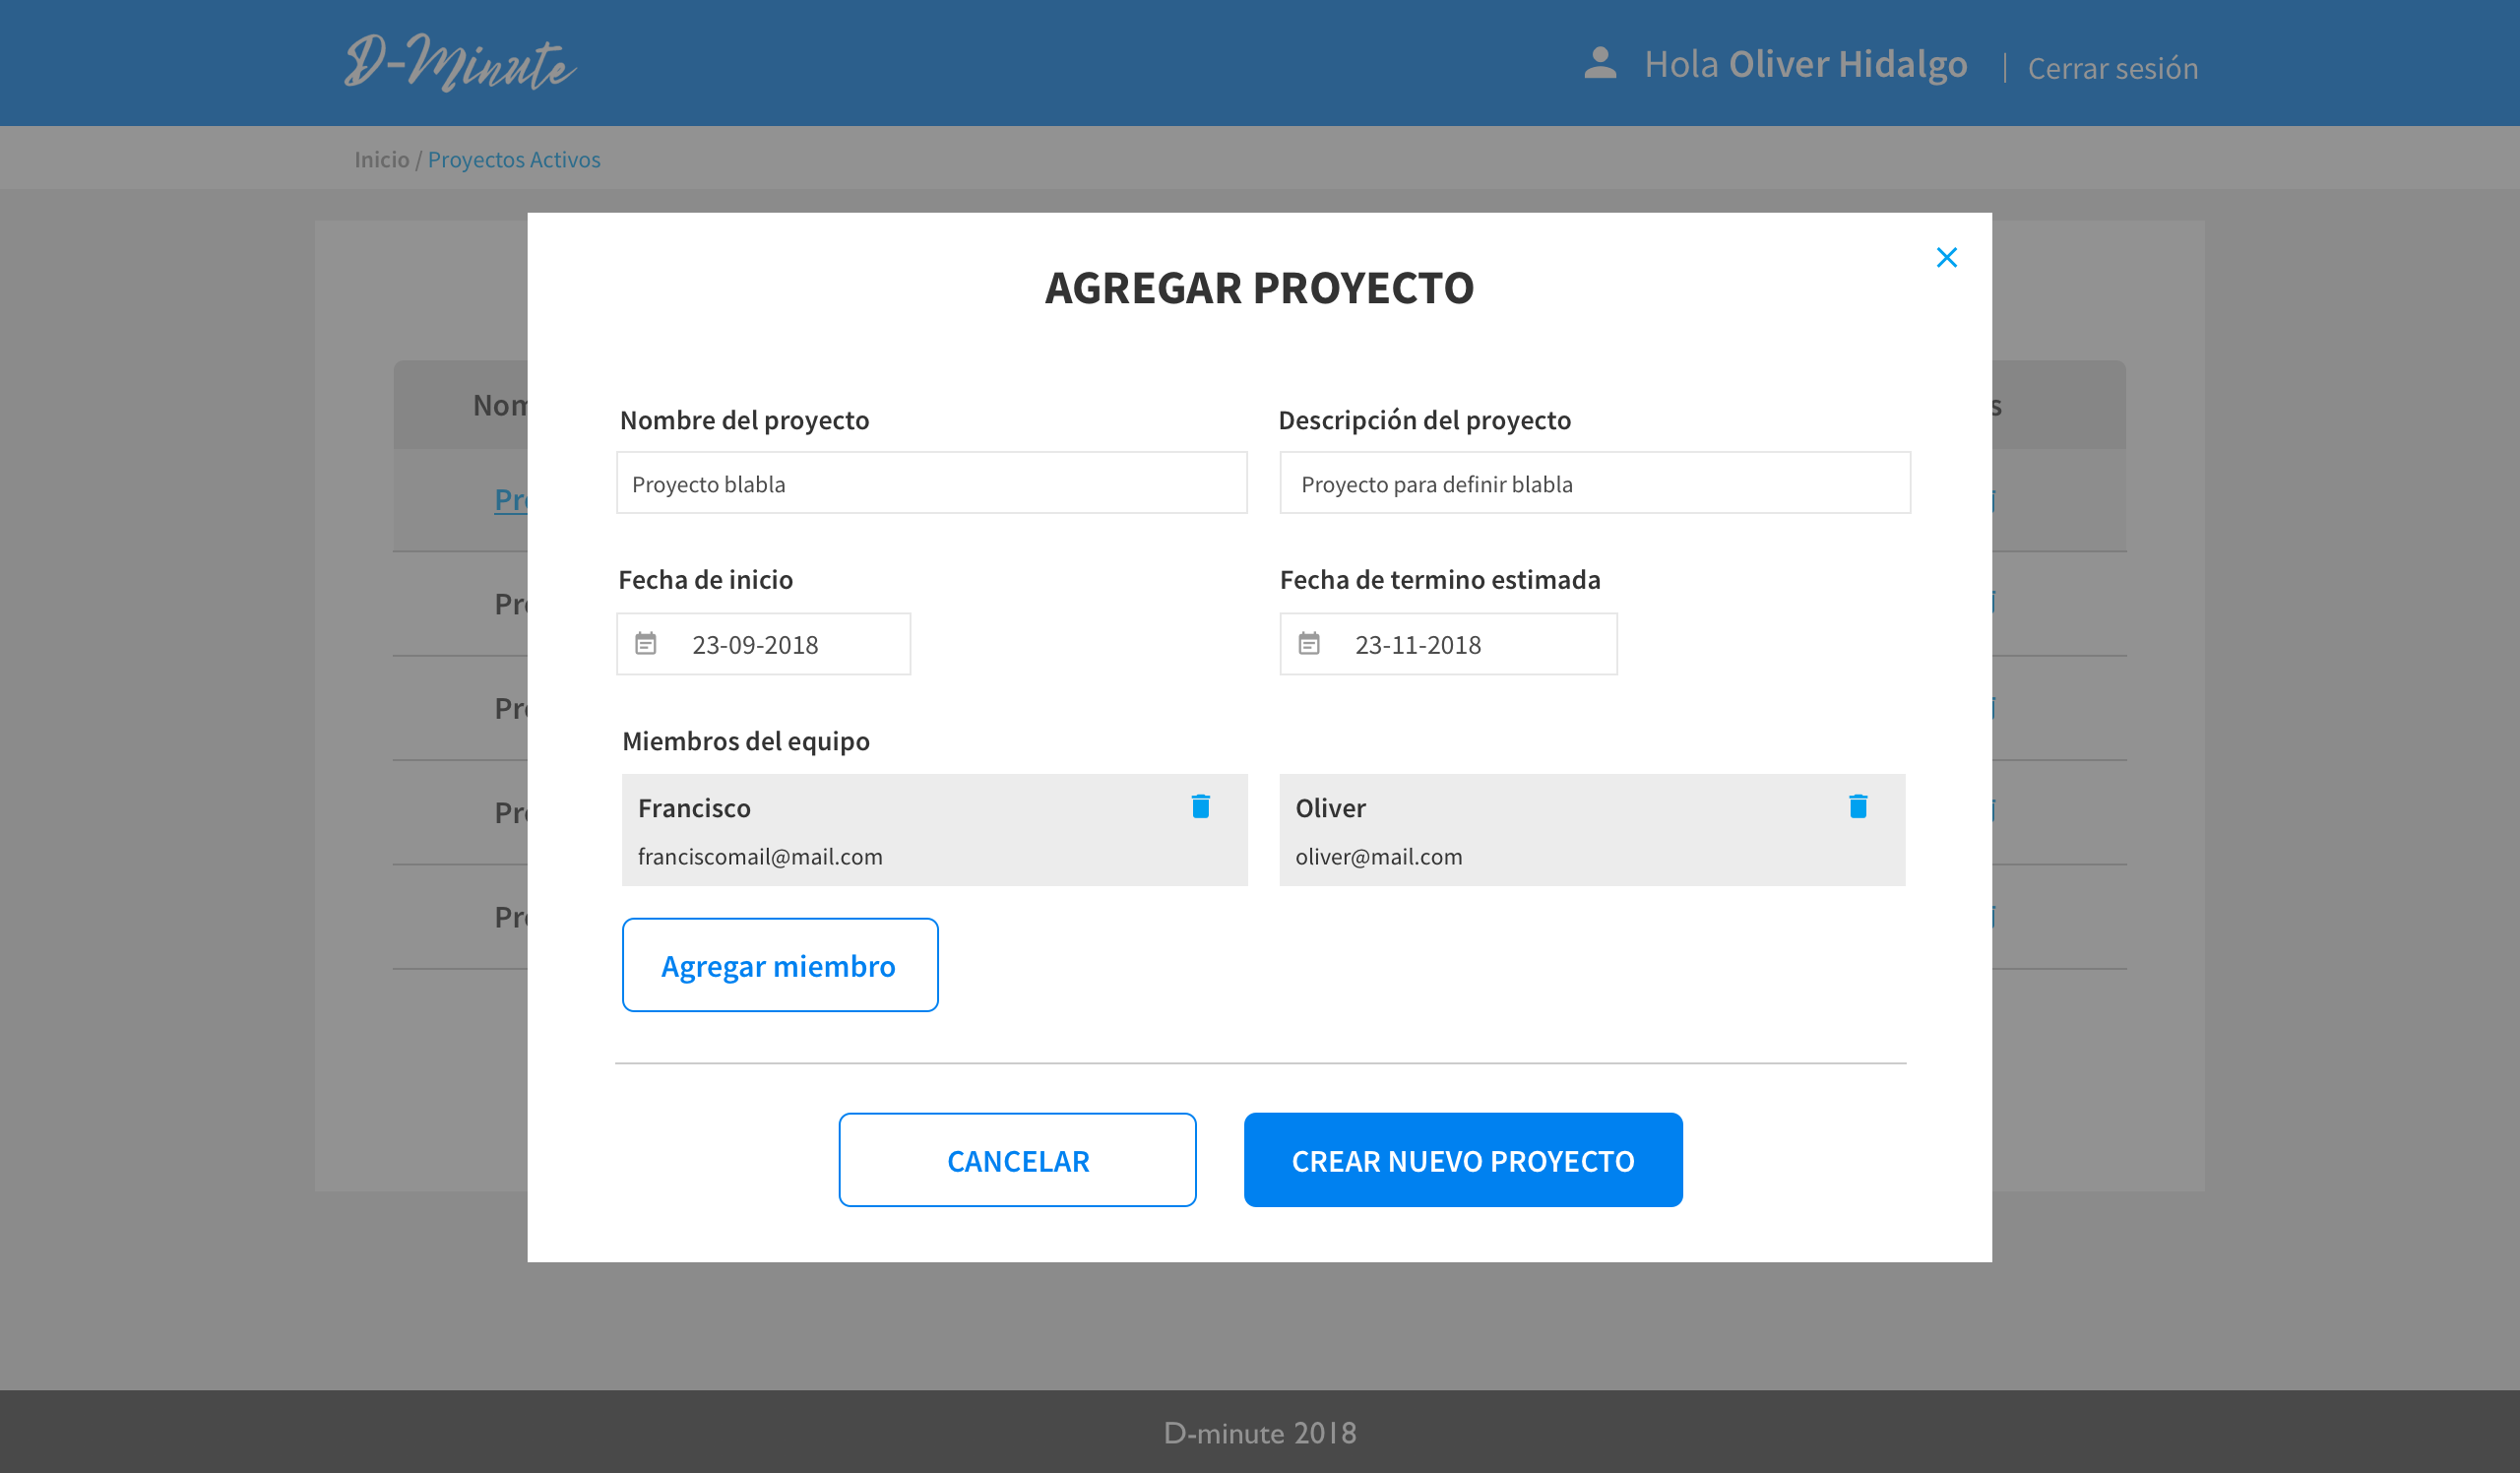
\includegraphics[width=11cm]{/app/Modal_agregarproyecto}
\caption{Diseño UX crear proyecto D-Minute; elaboración propia} 
\label{img4-8}
\end{figure}

La siguiente figura corresponde al listar proyectos activos, dado que lo importante es testear el producto y no desarrollar el 100\% de funcionalidades. Lo que agrega más valor es sólo ver los proyectos activos (ver figura \ref{img4-9}).

\begin{figure}[!h]
\centering
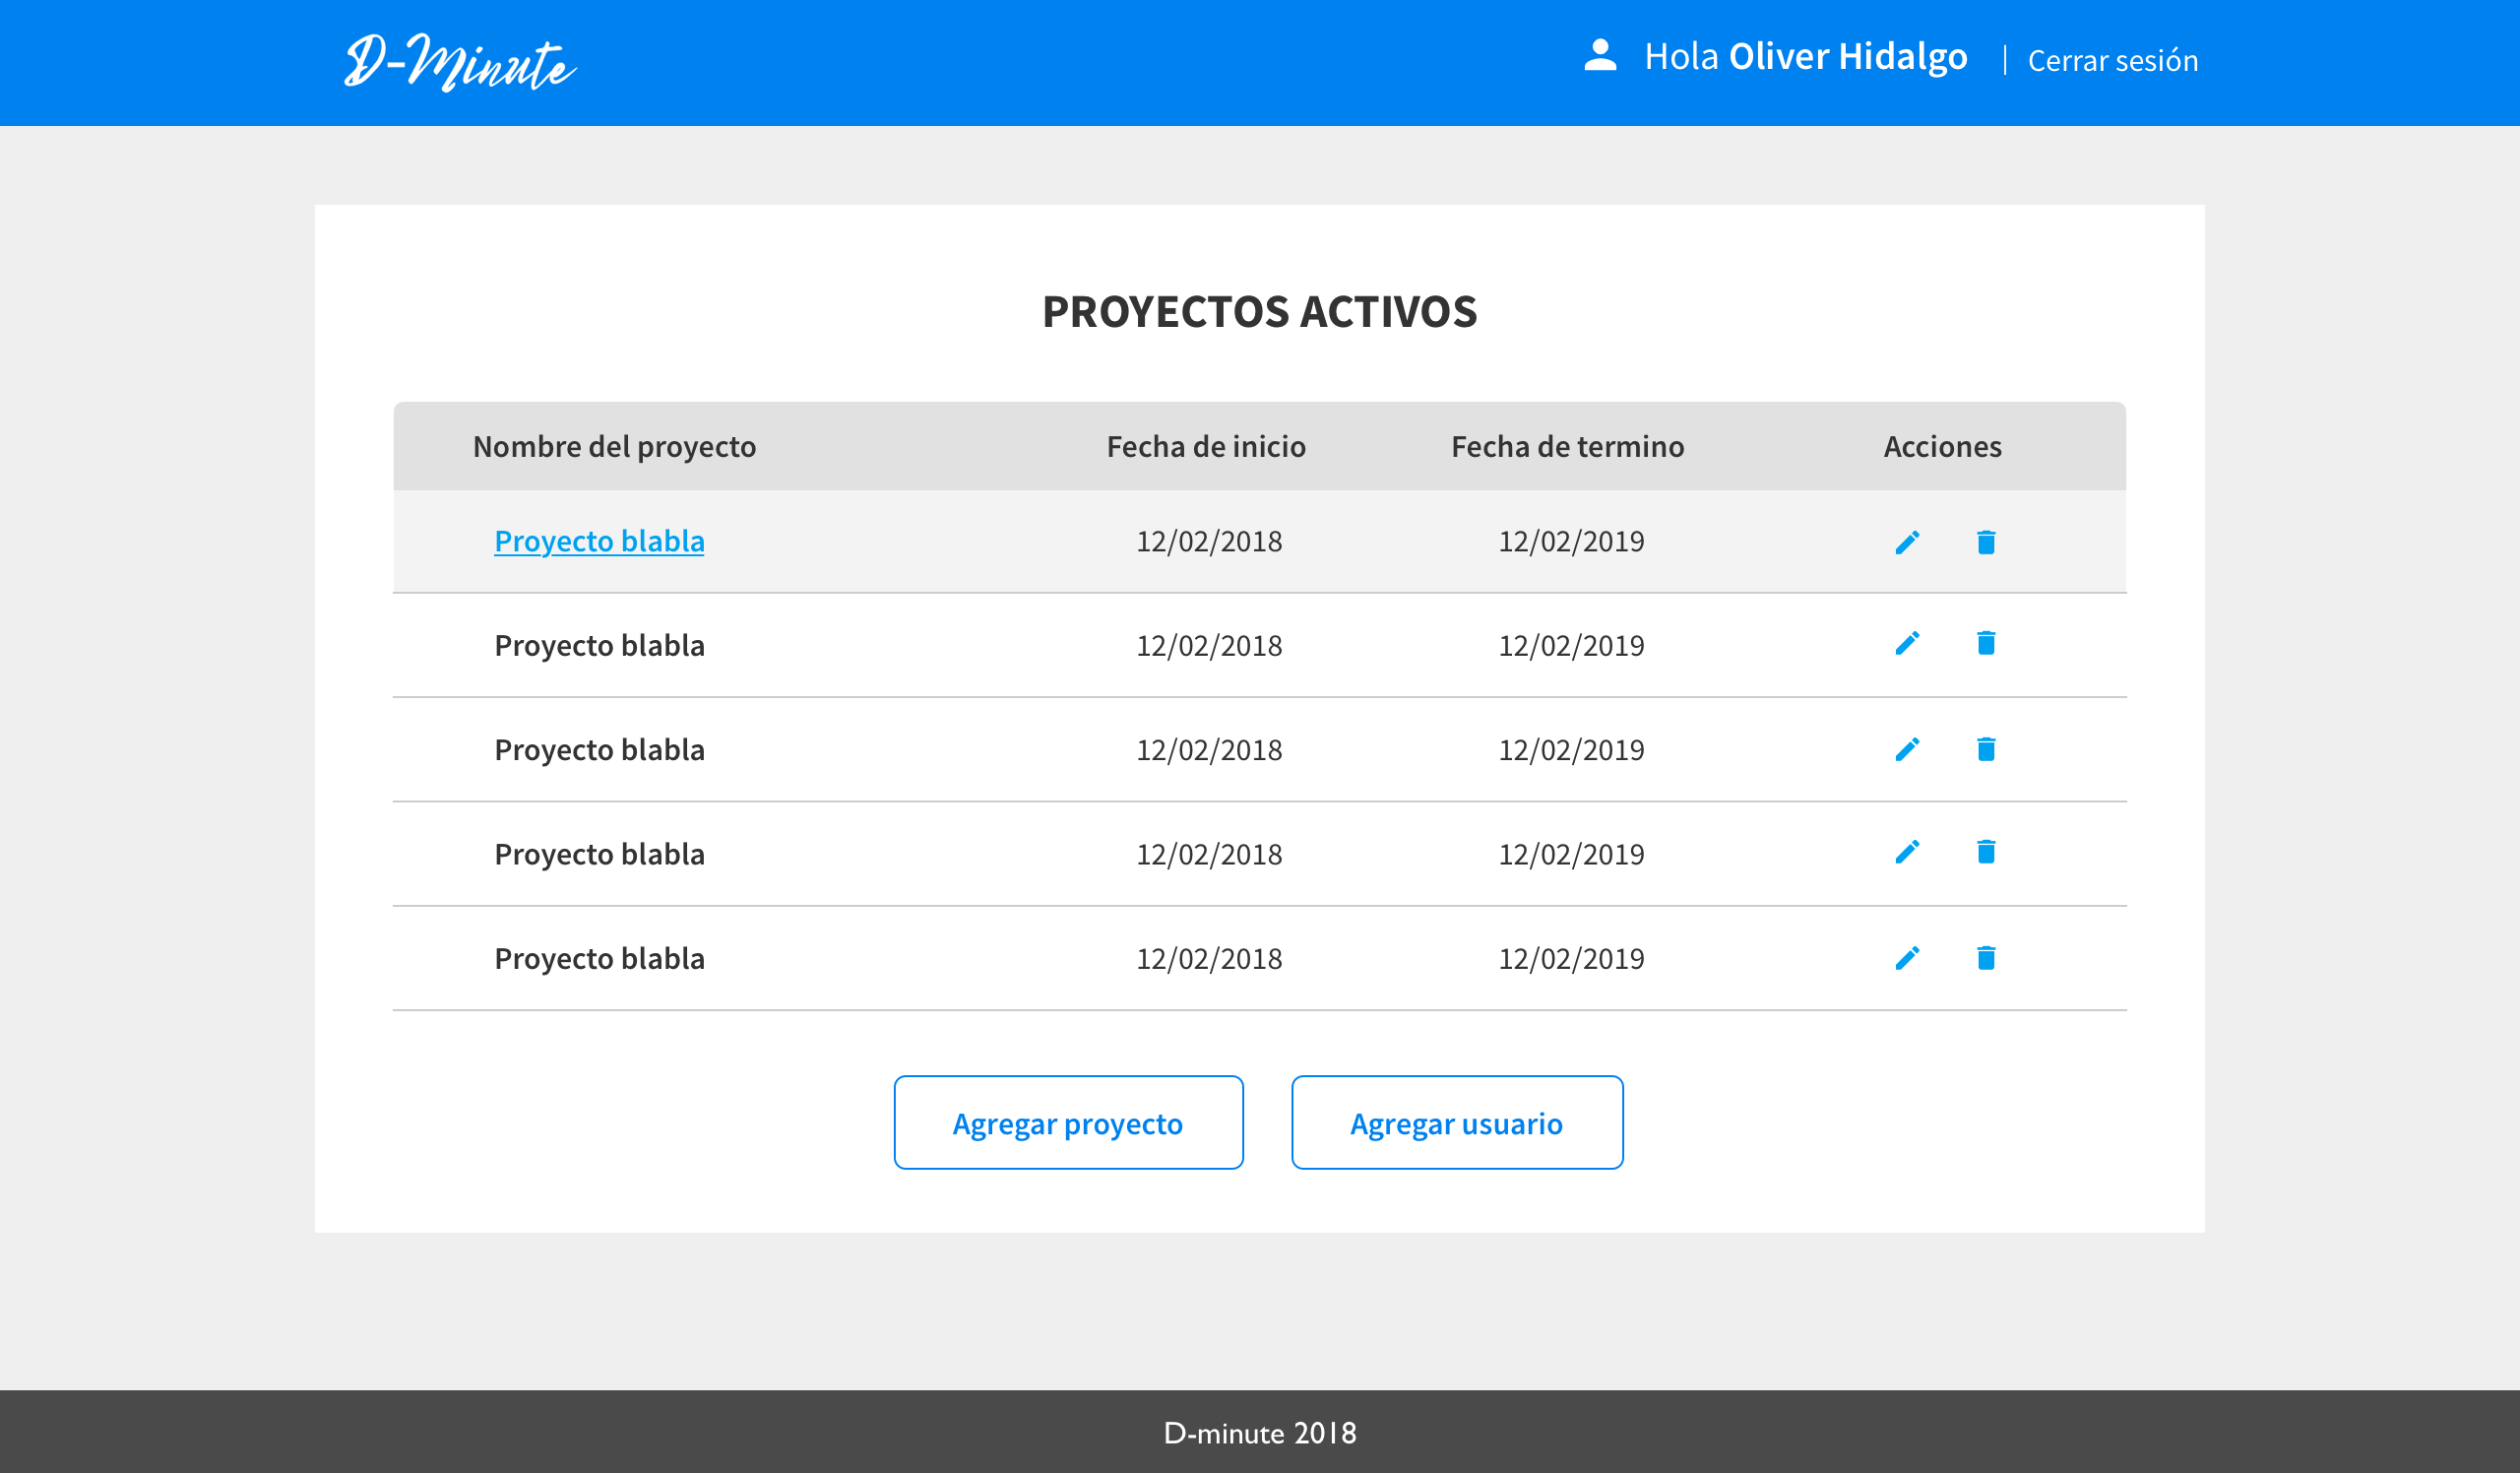
\includegraphics[width=11cm]{/app/Proyectos_Activos}
\caption{Diseño UX listar proyectos D-Minute; elaboración propia} 
\label{img4-9}
\end{figure}

Siguiendo la misma línea de dise\~no, la figura que sigue representa cómo se vería la opción agregar reunión o acta a un proyecto activo (ver figura \ref{img4-10}).

\begin{figure}[!h]
\centering
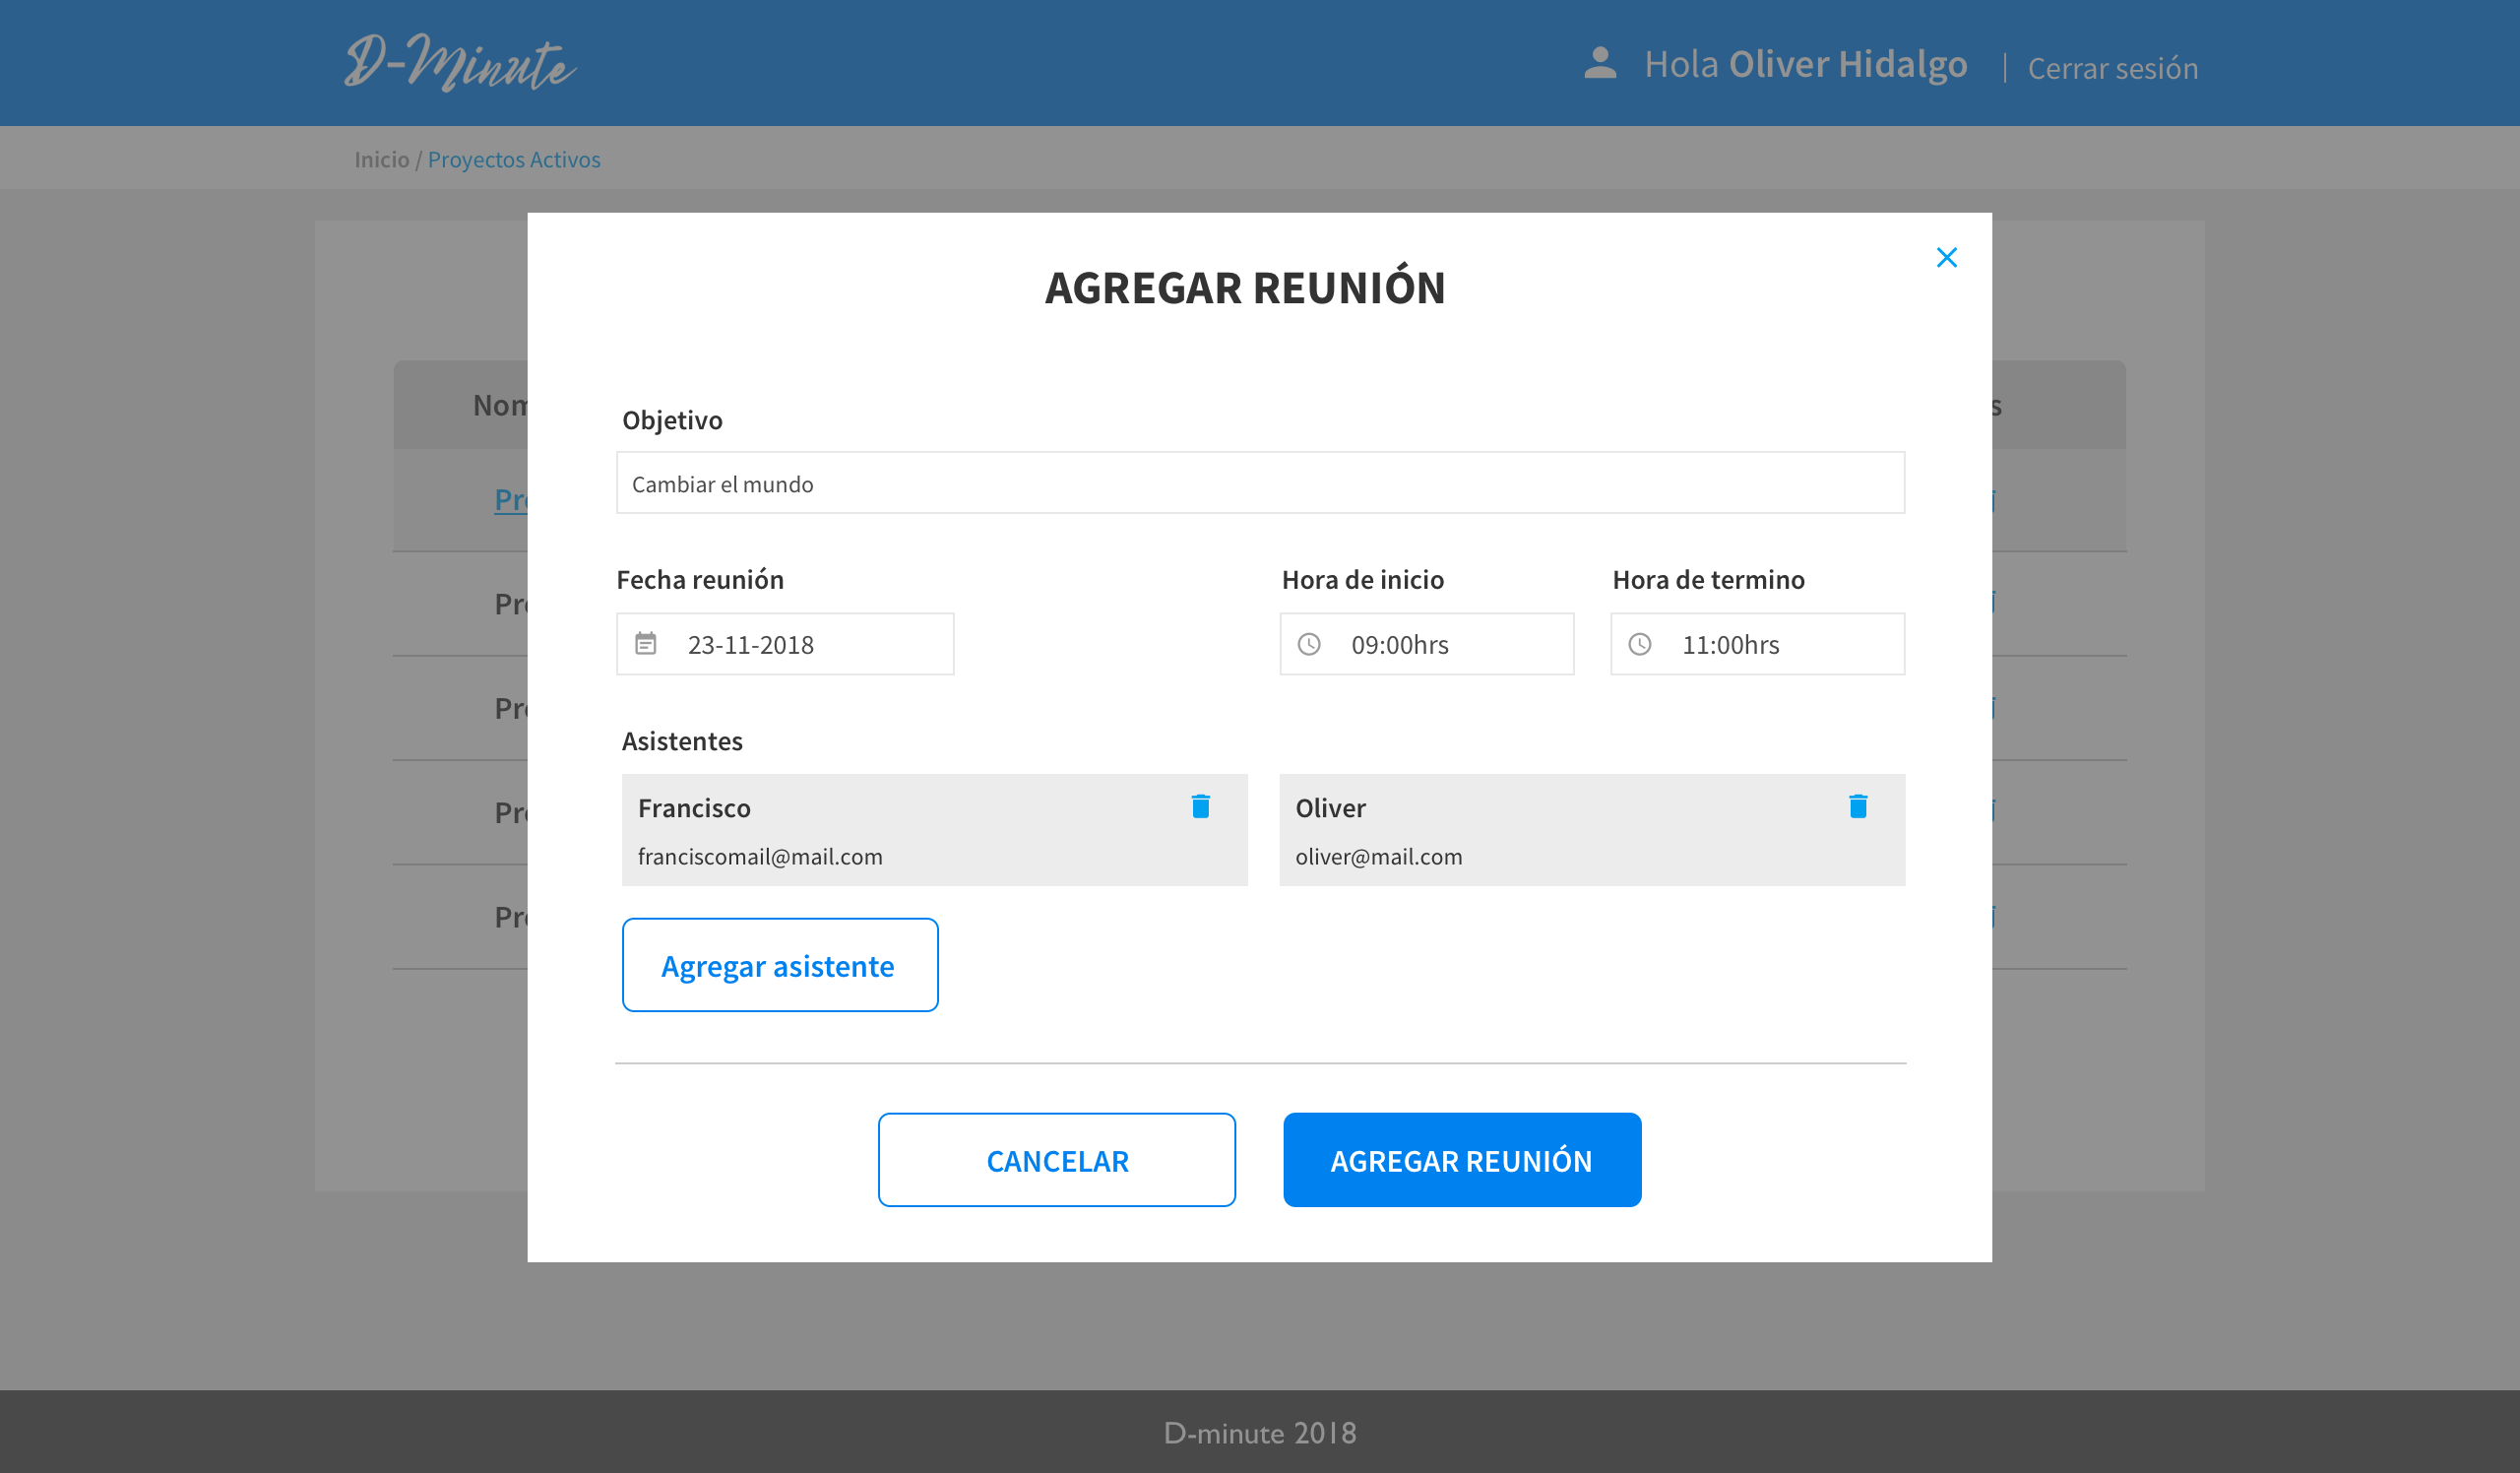
\includegraphics[width=11cm]{/app/Modal_Agregarreu}
\caption{Diseño UX crear acta D-Minute; elaboración propia} 
\label{img4-10}
\end{figure}

La siguiente figura representa el mockup inicial, luego de haber definido la línea gráfica que tendrá la aplicación, dicha figura expone las reuniones o actas que se desarrollan en el transcurso de un proyecto, sus temas y acciones asociadas (ver figura \ref{img4-11}).

\begin{figure}[!h]
\centering
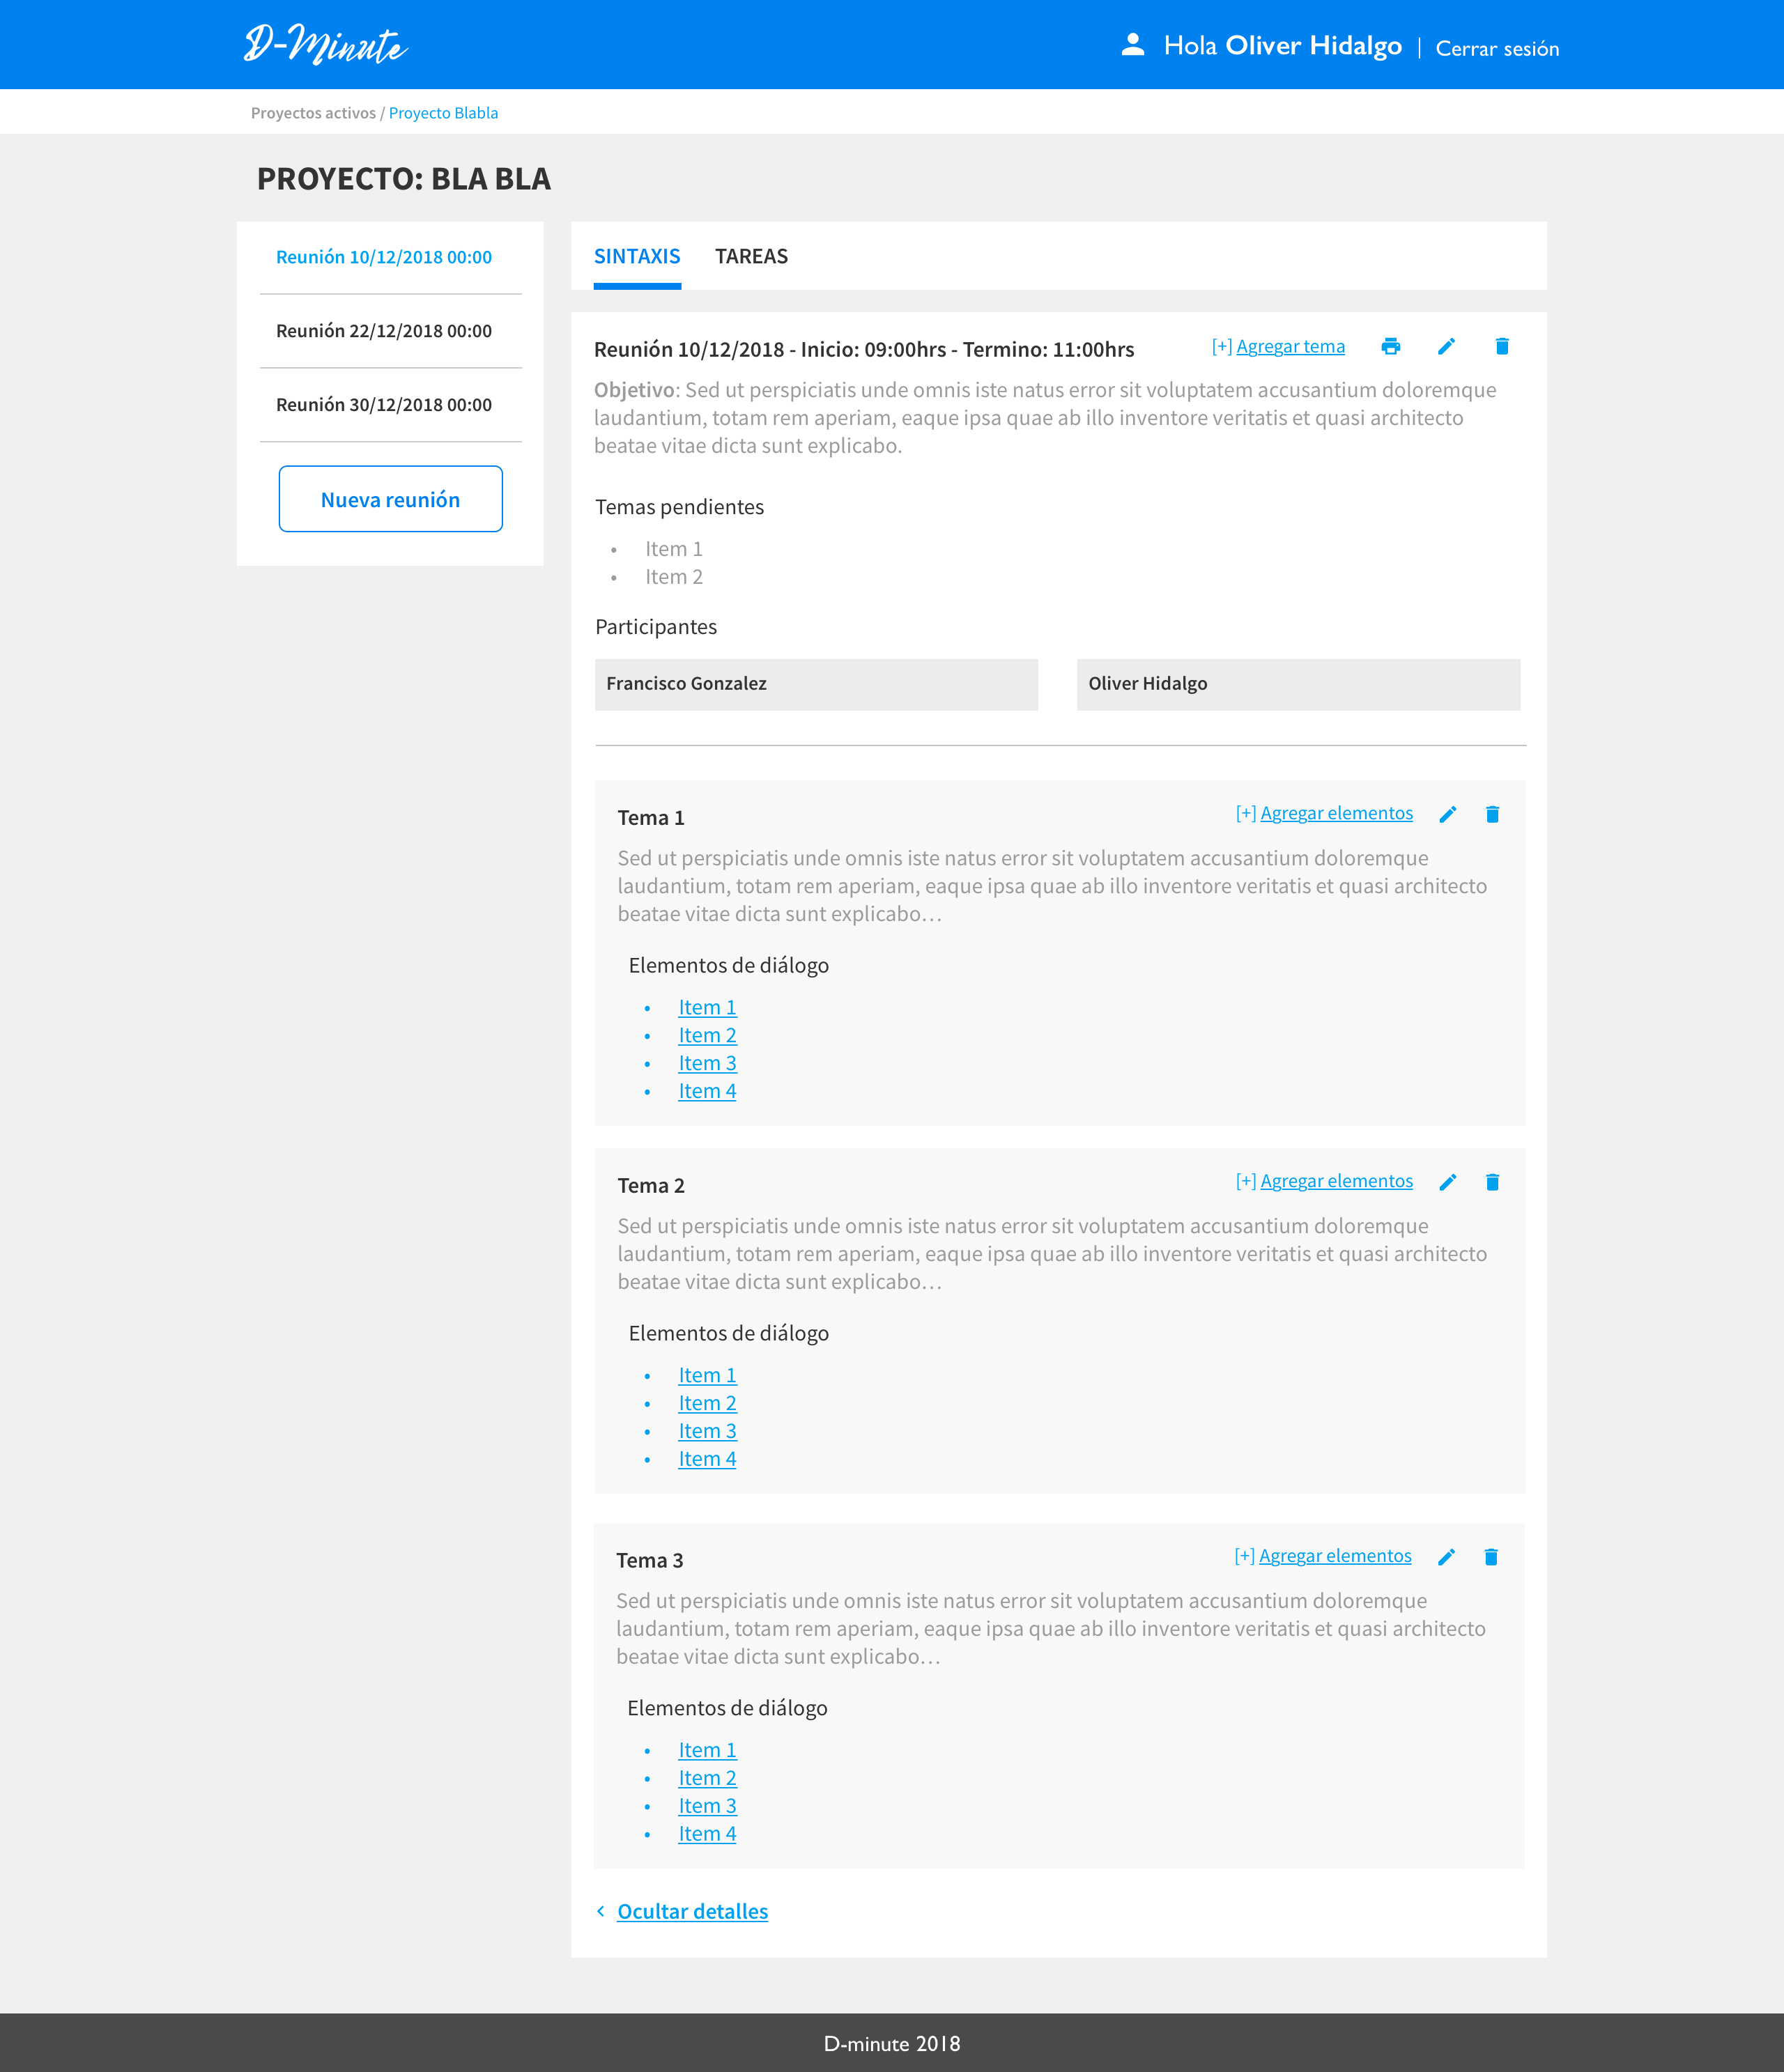
\includegraphics[width=13cm]{/app/despliegue}
\caption{Diseño UX reuniones de trabajo D-Minute; elaboración propia} 
\label{img4-11}
\end{figure}

Uno de los puntos más relevantes representados en la siguiente figura, tiene relación con agregar los elementos de diálogos - duda, acuerdo, compromiso, desacuerdo y norma - a un tema que es parte de una reunión de trabajo (ver figura \ref{img4-12}).

\begin{figure}[!h]
\centering
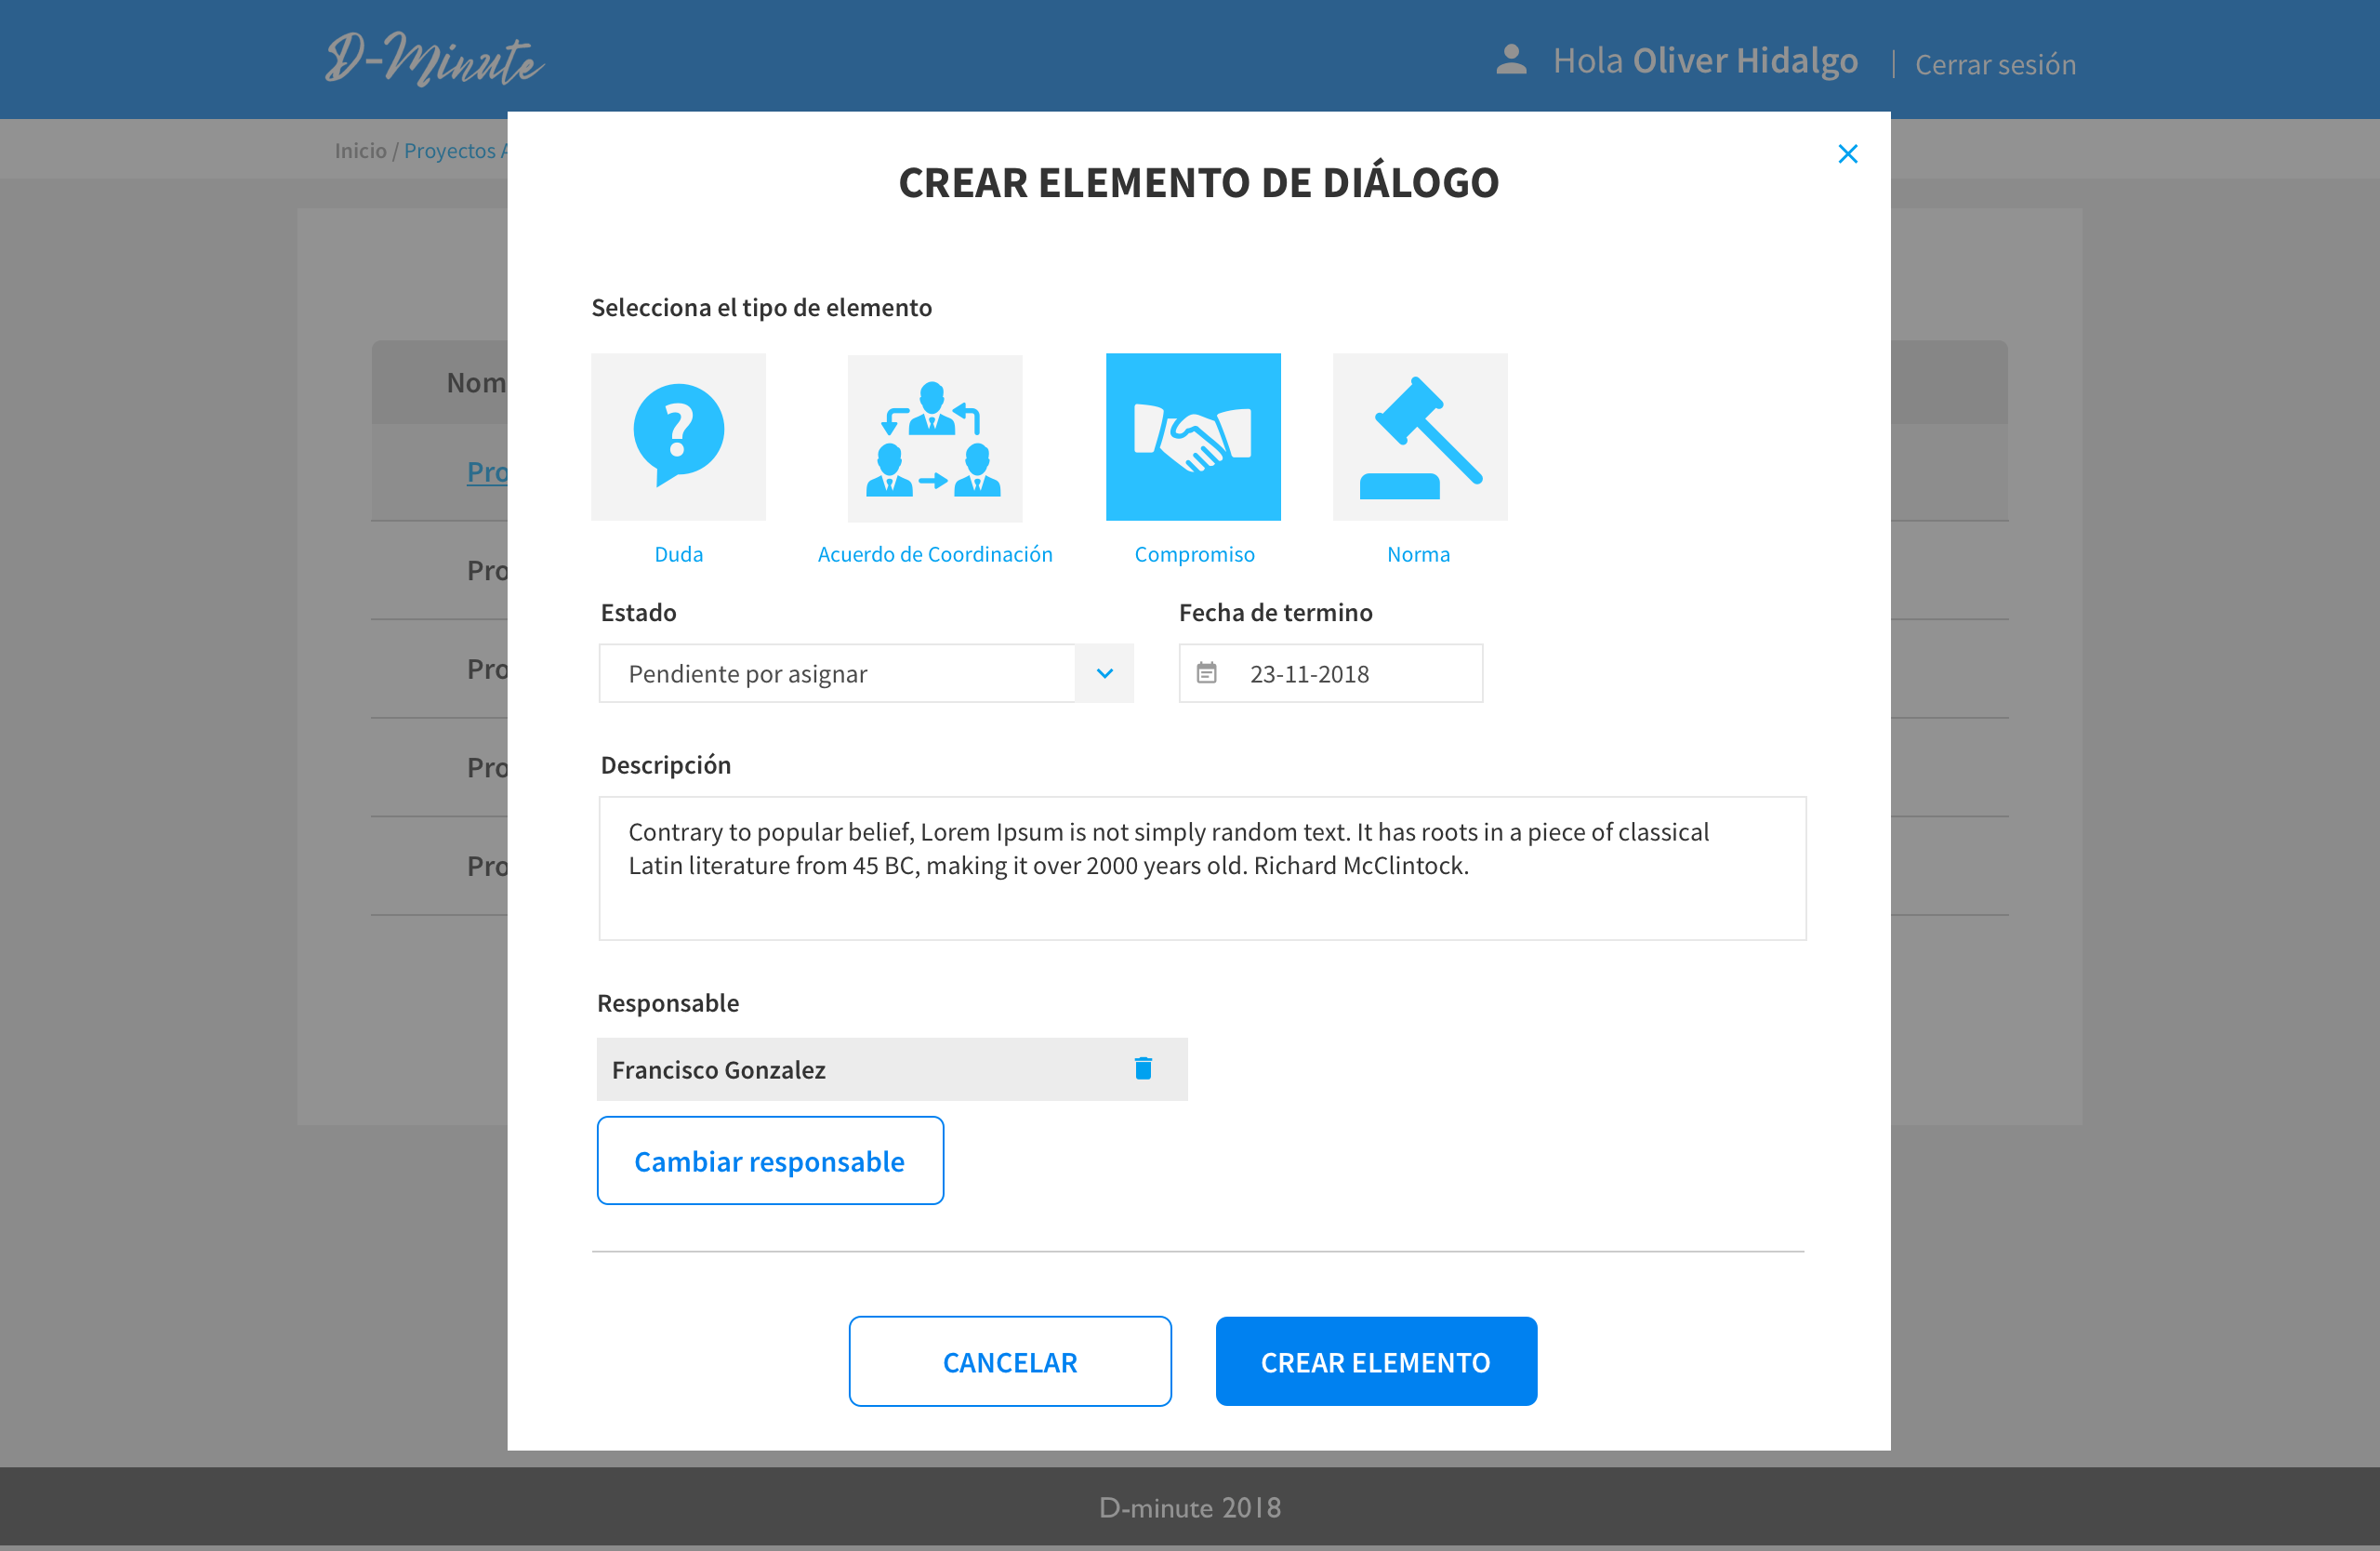
\includegraphics[width=11cm]{/app/Modal_Elemento_select_}
\caption{Diseño UX agregar elemento de diálogo D-Minute; elaboración propia} 
\label{img4-12}
\end{figure}

Por último con el fin de dar trazabilidad a los elementos, la siguiente figura representa las acciones que tiene un proyecto en un tablero de tareas (ver figura \ref{img4-13}).

\begin{figure}[!h]
\centering
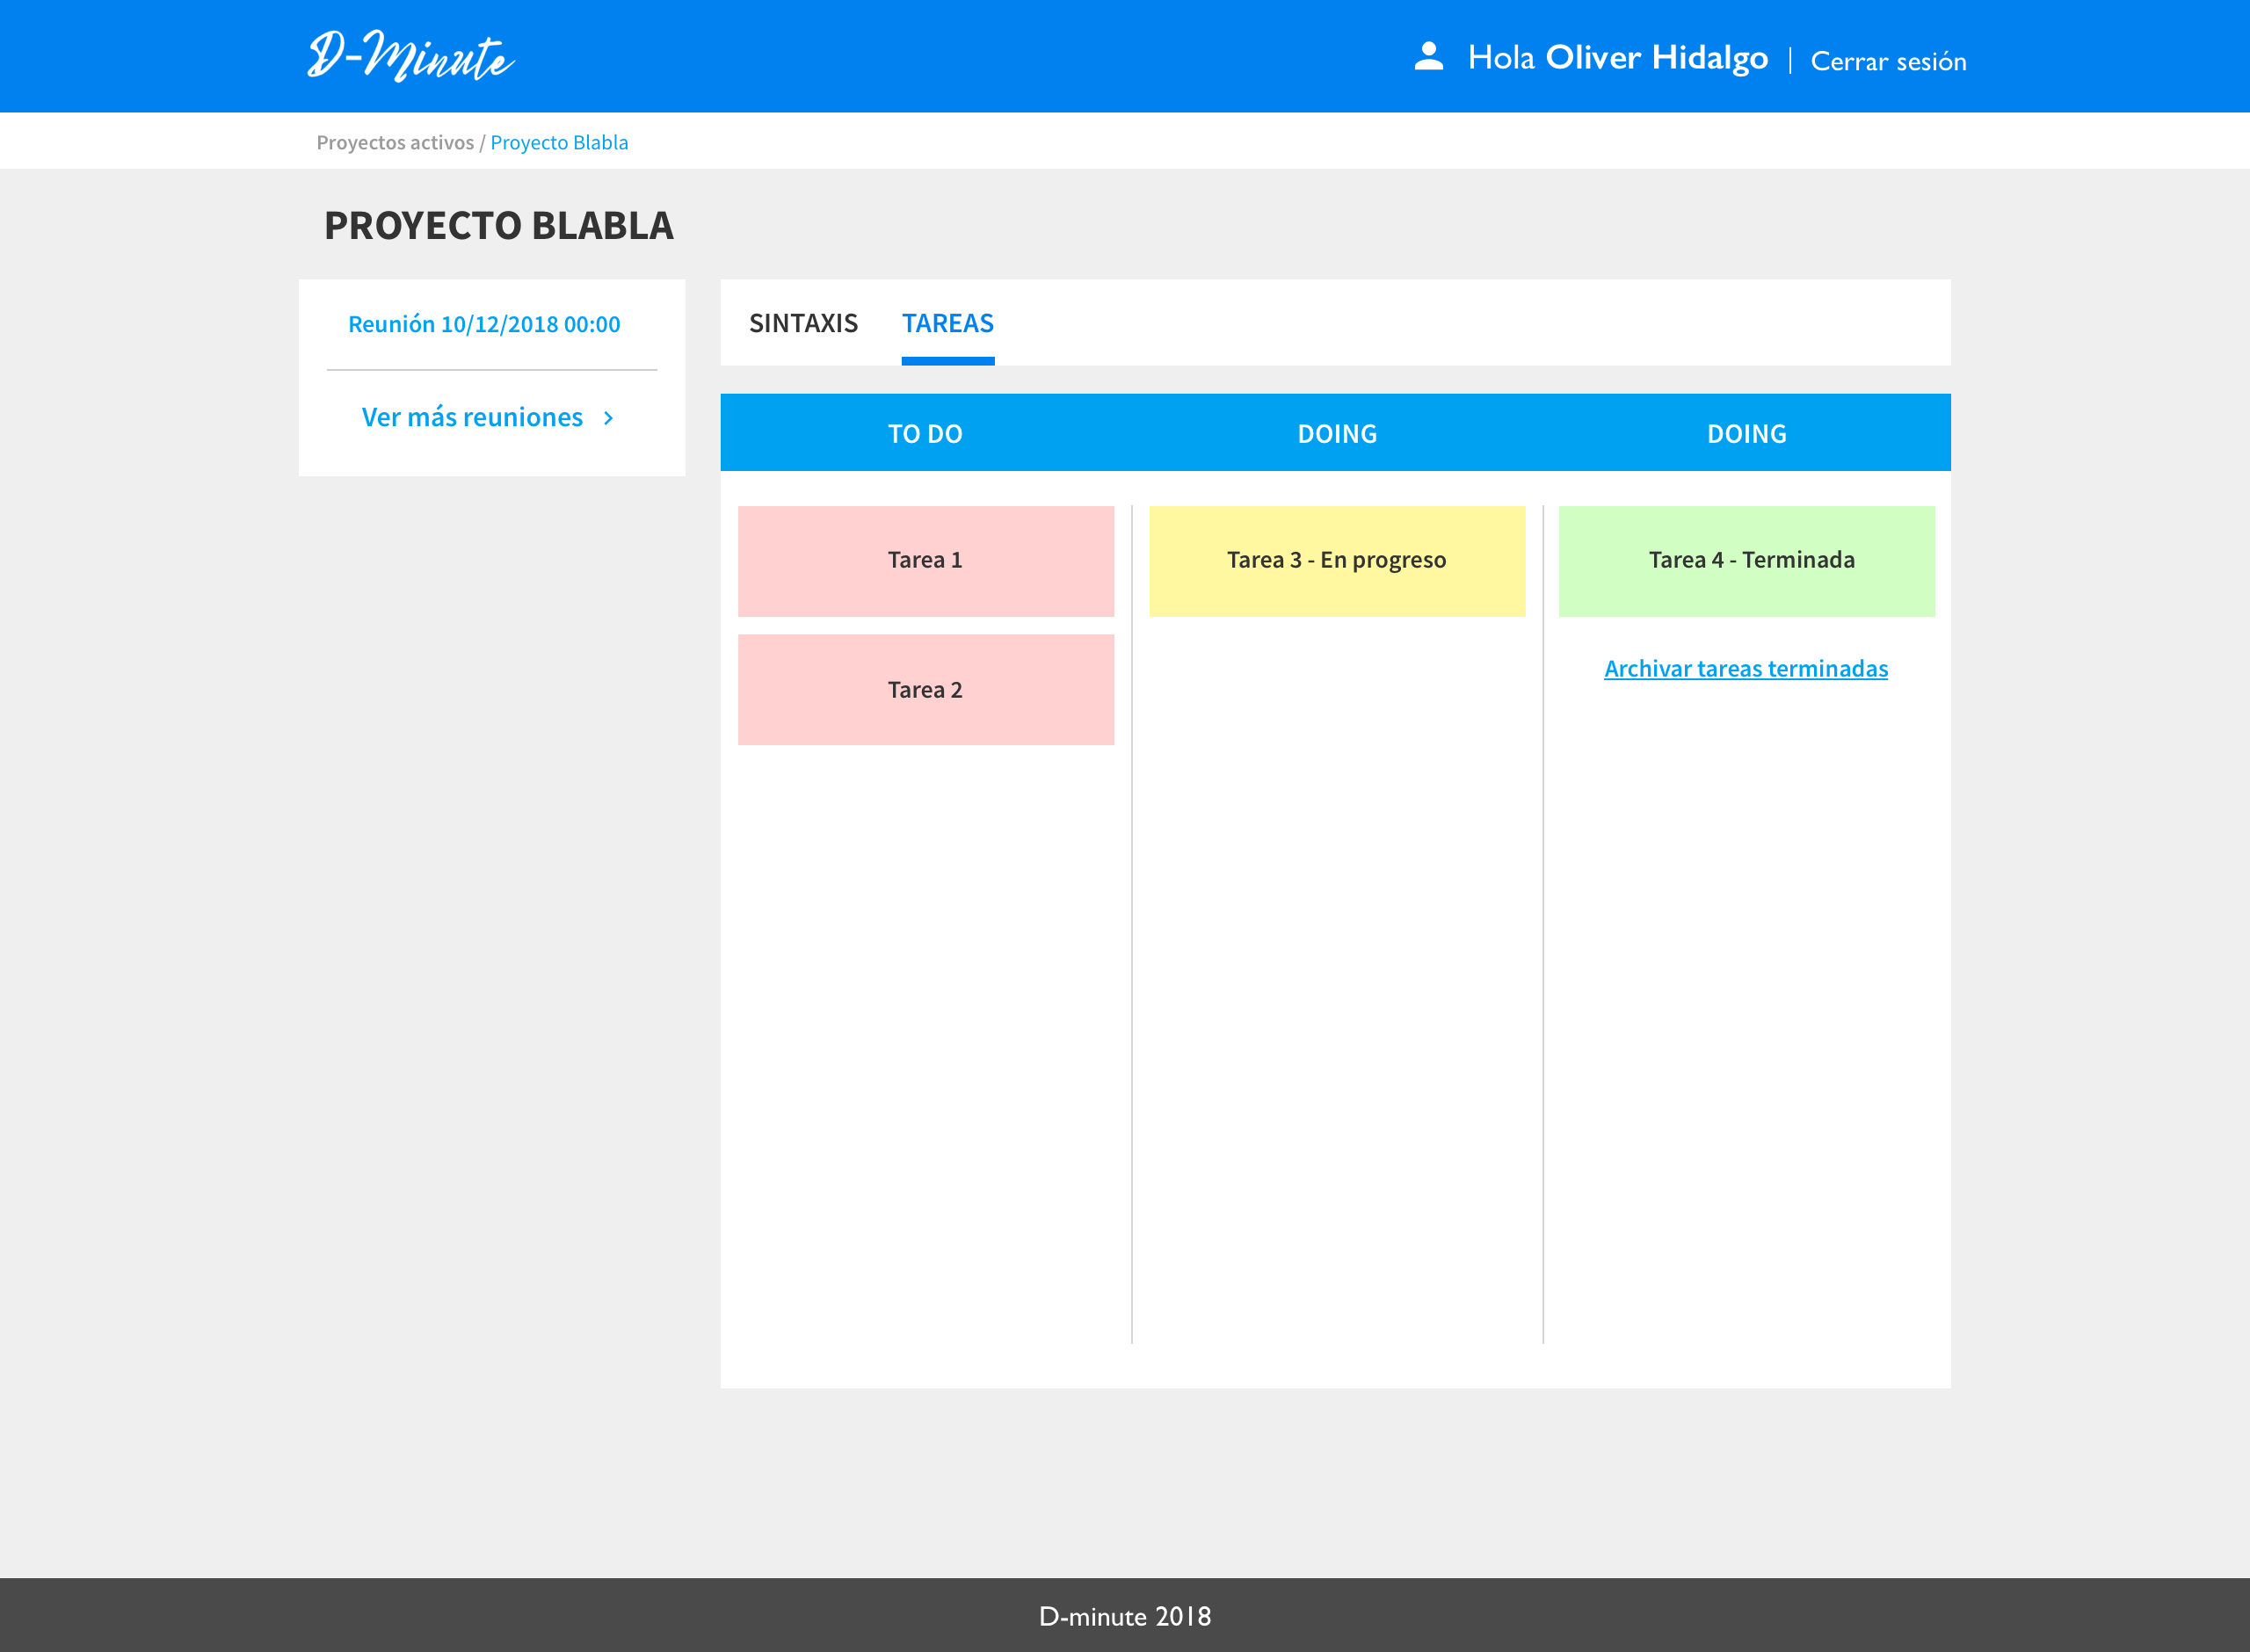
\includegraphics[width=11cm]{/app/tareas}
\caption{Diseño UX Kanban de tareas D-Minute; elaboración propia} 
\label{img4-13}
\end{figure}

\subsection{ARQUITECTURA}

\subsubsection{\textit{Front-End}}

Para el desarrollo de la parte \textit{front-end} se acuerda trabajar con \textbf{Angular 5} dado sus ventajas\footnote{Ver ventajas en: \url{https://www.campusmvp.es/recursos/post/angular-5-todo-lo-que-necesitas-saber-en-10-minutos-o-menos.aspx}} sobre otros lenguajes de programación y la velocidad que se puede dar al desarrollo trabajando con \textit{mockups} para no depender del \textit{back-end}. Lo anterior, sumado a la expertise del equipo sobre este \textit{framework}.

\subsubsection{\textit{Back-End}}

Para el desarrollo de la parte \textit{back-end} se acuerda trabajar microservicios en \textbf{Spring Boot} con java 1.8 utilizando maven como repositorio de librerías \textit{Release}. \textit{Spring} es uno de los framework que más esta siendo utilizados\footnote{Ver beneficios en : \url{https://es.linkedin.com/pulse/porque-me-gusta-trabajar-con-arquitectura-de-spring-boot-danilo-rodas
}} hoy en día por la gran cantidad de beneficios que ofrece: documentación, gestión de dependencias, fácil administración, entro otros factores\footnote{Ventajas: \url{https://code.i-harness.com/es/q/1b7eef7}} al momento de generar el desarrollo

\subsubsection{Base Dato}

Como gestor de datos se acuerda trabajar con MySQL en su versión 5.0 debido a que es una base datos \textit{opensource} con un excelente rendimiento y se acopla bastante bien con aplicación en la nube. 
El modelo no puede ser presentado debido a que a medida que se va construyendo el \textit{software} se va definiendo lo que se necesita con el fin de no gastar tiempo en cosas que no aportan valor.

\subsubsection{\textit{Platform as a Service (Paas)}}

Dado que el desarrollo de D-Minute será llevado a cabo en micro arquitectura, se acuerda utilizar Heroku\footnote{Heroku: \url{https://es.wikipedia.org/wiki/Heroku}} como Paas en la nube. Debido a que su servicio gratuito ofrece muchas ventajas para el despliegue y seguimiento de la aplicación como también un soporte para alta disponibilidad (ver figura \ref{img4-14}).

De igual forma forma el sistema fue instalado en un servidor del Departamento de Ingeniería Informática de la USACH utilizando Docker para el despliegue de la arquitectura digital.

\begin{figure}[!h]
\centering
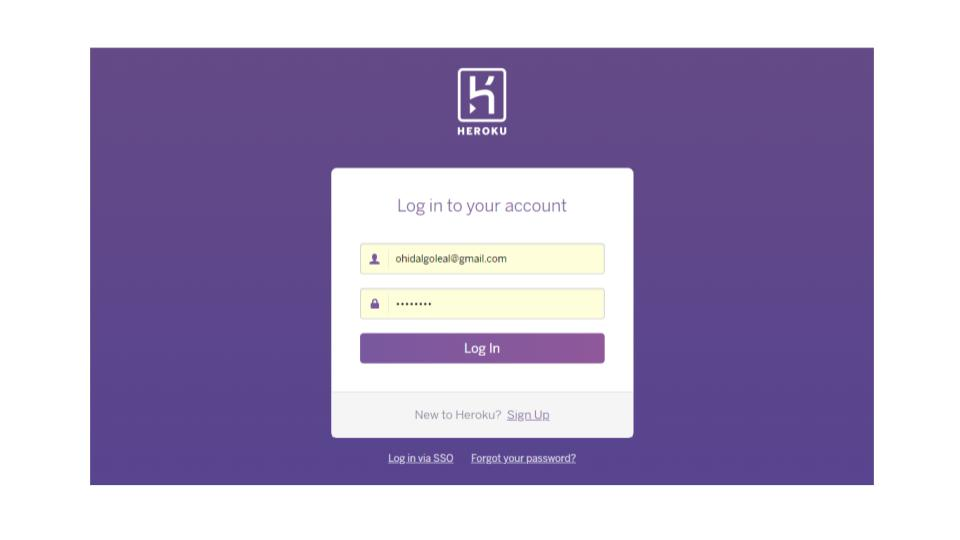
\includegraphics[width=11cm]{/heroku}
\caption{PaaS Heroku; tomado de Heroku} 
\label{img4-14}
\end{figure}

\subsubsection{Diagrama de Arquitectura}

El siguiente diagrama de arquitectura fue acordado con el equipo para dar a conocer la forma que será abordado el desarrollo y tener una visión general de cómo estará construido el producto (ver figura \ref{img4-15}).

\begin{figure}[!h]
\centering
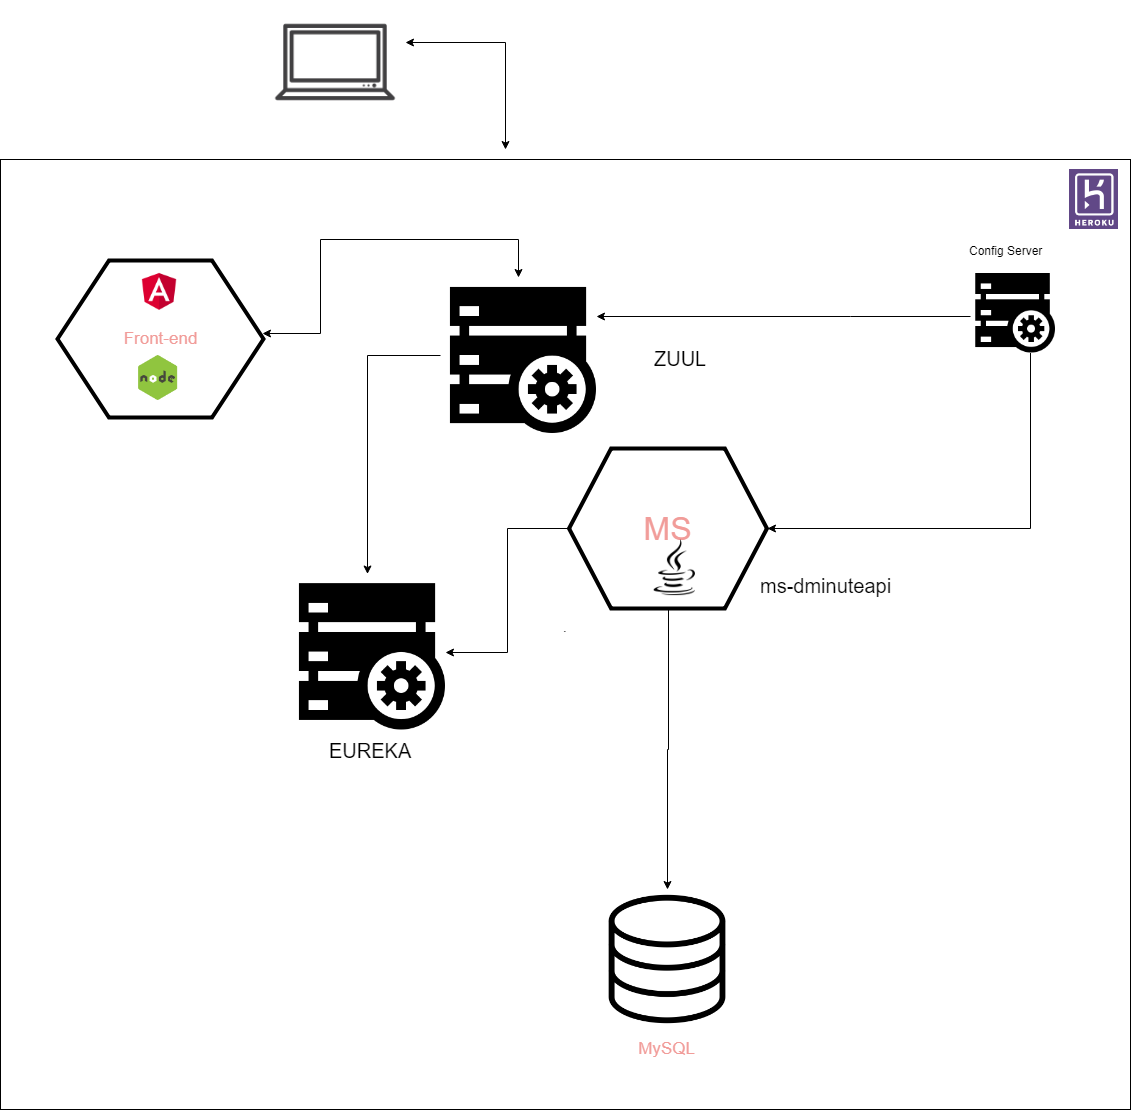
\includegraphics[width=11cm]{/disenioArquitectura}
\caption{Dise\~no Arquitectura D-Minute; elaboración propia} 
\label{img4-15}
\end{figure}

\subsection{DESARROLLO PRODUCTO EN \textit{SPRINT}}

A continuación se detalle el desarrollo del producto en \textit{sprint} y las historias de usuario comprometidas:

\begin{itemize}
	\item \textbf{\textit{Sprint} 1:} Configurar ambientes para desarrollo. Ver \textit{spring backlog} en tabla \ref{tab:backlog1}

\begin{table}[!h]
\centering
\caption{\textit{Sprint} uno, \textit{Sprint Backlog}: Preparar ambiente \textit{Developer}, Refactorización temas acta, elaboración propia}
\label{tab:backlog1}
\begin{tabular}{|l|l|r|}
\hline
\multicolumn{1}{|c|}{\textit{\textbf{Feature}}} & \textbf{Epica} & \textbf{Peso} \\ \hline
Configuración ambiente DMinute & Técnica & 3 \\ \hline
Levantar aplicación web en Heroku & Técnica & 3 \\ \hline
Refactorización de código para creación de temas de la reunión & Técnica & 8 \\ \hline
\end{tabular}
\end{table}

	\item \textbf{\textit{Sprint} 2:} Desarrollar APIs de servicios para la creación de actas y elementos de diálogo. Ver \textit{spring backlog} en tabla \ref{tab:backlog2}

\begin{table}[!h]
\centering
\caption{\textit{Sprint} dos, \textit{Sprint Backlog}: Refactorización acta y elementos de diálogo, elaboración propia}
\label{tab:backlog2}
\begin{tabular}{|l|l|r|}
\hline
\multicolumn{1}{|c|}{\textit{\textbf{Feature}}} & \textbf{Epica} & \textbf{Peso} \\ \hline
Refactorización de código para creación elementos de diálogo & Técnica & 8 \\ \hline
Refactorización de código para creación de minutas & Técnica & 8 \\ \hline
\end{tabular}
\end{table}

	\item \textbf{\textit{Sprint} 3:} Generar estructura de proyecto \textit{front-end} en angular 5. Ver \textit{spring backlog} en tabla \ref{tab:backlog3}

\begin{table}[!h]
\centering
\caption{\textit{Sprint} tres, \textit{Sprint Backlog}: Refactorización acta y elementos de diálogo, elaboración propia}
\label{tab:backlog3}
\begin{tabular}{|l|l|r|}
\hline
\multicolumn{1}{|c|}{\textit{\textbf{Feature}}} & \textbf{Epica} & \textbf{Peso} \\ \hline
Implementación nueva estructura UX & Técnica & 8 \\ \hline
Eliminar envio de correo en creación usuario & Técnica & 3 \\ \hline
Cambiar librería de input de textos & Generación Acta & 3 \\ \hline
\textit{Spike} -  Revisar librería Kanban tareas & Seguimiento de tareas & 2 \\ \hline
\end{tabular}
\end{table}

	\item \textbf{\textit{Sprint} 4:} Migrar por completa aplicación de python a microarquitectura e implementar modelo final de base datos. Ver \textit{spring backlog} en tabla \ref{tab:backlog4}

\begin{table}[!h]
\centering
\caption{\textit{Sprint} cuatro, \textit{Sprint Backlog}: Reestructurar menú actas y listar acta, elaboración propia}
\label{tab:backlog4}
\begin{tabular}{|l|l|r|}
\hline
\multicolumn{1}{|c|}{\textit{\textbf{Feature}}} & \textbf{Epica} & \textbf{Peso} \\ \hline
Reestructurar Menú Creación de Actas & Evolución UX & 5 \\ \hline
Reestructurar Listado de Minutas & Evolución UX & 8 \\ \hline
\end{tabular}
\end{table}

	\item \textbf{\textit{Sprint} 5:} Implementar modelo de micro servicios en \textit{cloud} y generar estilos estándar de la aplicación. Ver \textit{spring backlog} en tabla \ref{tab:backlog5}

\begin{table}[!h]
\centering
\caption{\textit{Sprint} cinco, \textit{Sprint Backlog}: Visualizar detalle minuta y normalizar estilos, elaboración propia}
\label{tab:backlog5}
\begin{tabular}{|l|l|r|}
\hline
\multicolumn{1}{|c|}{\textit{\textbf{Feature}}} & \textbf{Epica} & \textbf{Peso} \\ \hline
Normalizar colores aplicación & Evolución UX & 5 \\ \hline
Cargar usuarios nuevos al crear un proyecto & Generación Acta & 5 \\ \hline
Visualizar detalle minuta & Evolución UX & 8 \\ \hline
\end{tabular}
\end{table}


	\item \textbf{\textit{Sprint} 6:} Mejorar aspectos visuales de la aplicación arrastrados de la migración. Ver \textit{spring backlog} en tabla \ref{tab:backlog6}

\begin{table}[!h]
\centering
\caption{\textit{Sprint} seis, \textit{Sprint Backlog}: Eliminación menú y mejoras visuales, elaboración propia}
\label{tab:backlog6}
\begin{tabular}{|l|l|r|}
\hline
\multicolumn{1}{|c|}{\textit{\textbf{Feature}}} & \textbf{Epica} & \textbf{Peso} \\ \hline
Texto al agregar elementos de diálogo & Generación Acta & 1 \\ \hline
Eliminación Menú & Evolución UX & 1 \\ \hline
BUG: editar un elemento de diálogo & Generación Acta & 3 \\ \hline
Quitar opción colapsable & Evolución UX & 5 \\ \hline
Nombre en barra superior & Evolución UX & 2 \\ \hline
Calendario en español & Generación Acta & 3 \\ \hline
\end{tabular}
\end{table}


	\item \textbf{\textit{Sprint} 7:} Implementar nuevo diseño UX y corrección de \textit{bugs} críticos. Ver \textit{spring backlog} en tabla \ref{tab:backlog7}

\begin{table}[!h]
\centering
\caption{\textit{Sprint} siete, \textit{Sprint Backlog}: Incorporación nuevos iconos y BUG producción, elaboración propia}
\label{tab:backlog7}
\begin{tabular}{|l|l|r|}
\hline
\multicolumn{1}{|c|}{\textit{\textbf{Feature}}} & \textbf{Epica} & \textbf{Peso} \\ \hline
BUG: seleccionar asistentes de una reunión & Generación Acta & 5 \\ \hline
BUG: al editar y crear un acta & Generación Acta & 5 \\ \hline
Mejora estilo + iconos & Evolución UX & 8 \\ \hline
BUG: Se duplica acta al editar & Generación Acta & 5 \\ \hline
\end{tabular}
\end{table}


	\item \textbf{\textit{Sprint} 8:} Reducir deuda técnica de \textit{front-end} y \textit{back-end}. Ver \textit{spring backlog} en tabla \ref{tab:backlog8}

\begin{table}[!h]
\centering
\caption{\textit{Sprint} ocho, \textit{Sprint Backlog}: Mejoras al crear acta, selección icono al crear elemento de diálogo, elaboración propia}
\label{tab:backlog8}
\begin{tabular}{|l|l|r|}
\hline
\multicolumn{1}{|c|}{\textit{\textbf{Feature}}} & \textbf{Epica} & \textbf{Peso} \\ \hline
Seleccionar Icono al agregar elemento de diálogo & Trazabilidad Elementos & 8 \\ \hline
BUG: Se corta pantalla al agregar elemento de diálogo & Evolución UX & 3 \\ \hline
Quitar espaciado Panel de Proyecto & Evolución UX & 2 \\ \hline
Número reunión & Generación Acta & 5 \\ \hline
\end{tabular}
\end{table}

\end{itemize}

Para ver más en detalle el desarrollo del producto, ver anexo C de este mismo documento.

\subsection{RESUMEN}

El presente capítulo tuvo lugar el desarrollo del \textit{software}, recordemos que la tesis se compone de I+D, donde “D” corresponde al desarrollo. Si bien había expectativas por lograr construir todas las funcionalidades, al final se enfocaron los esfuerzos en un MVP del producto en base al \textit{release map} presentado.

Los puntos uno, dos y tres fueron desarrollados a nivel de épica y los puntos cuatro y cinco no se logró finalizar por falta de tiempo y prioridades del producto. Recordar que para el desarrollo del \textit{software} se utiliza la metodología ágil Scrum que minimiza la planificación y se enfoca en el prototipo.

Además de lo anterior, en este capítulo hubo un fuerte trabajo colaborativo para llevar a cabo: la migración de código python a java, el nuevo look and feel y el desarrollo en micro servicios en servidores \textit{cloud}.

En el próximo capítulo se presenta el diseño del experimento para validar las preguntas de investigación.
